%--------------------
% Packages
% -------------------
\documentclass[11pt,a4paper]{article}
\usepackage[utf8x]{inputenc}
\usepackage[T1]{fontenc}
%\usepackage{gentium}
\usepackage{mathptmx} % Use Times Font
% \usepackage{wordcount}
\usepackage{listings}
\usepackage{amsmath}
\usepackage{minted}
\usepackage{pdflscape}
\usepackage[pdftex]{graphicx} % Required for including pictures
\usepackage[pdftex,linkcolor=black,pdfborder={0 0 0}]{hyperref} % Format links for pdf
\usepackage{calc} % To reset the counter in the document after title page
\usepackage[numbers]{natbib}
\usepackage{amssymb} % Required for \mathbb
\usepackage{amsmath} % Required for bmatrix environment
\frenchspacing % No double spacing between sentences
\linespread{1.2} % Set linespace
\usepackage[a4paper, lmargin=0.1666\paperwidth, rmargin=0.1666\paperwidth, tmargin=0.1111\paperheight, bmargin=0.1111\paperheight]{geometry} %margins
%\usepackage{parskip}

\usepackage[all]{nowidow} % Tries to remove widows
\usepackage[protrusion=true,expansion=true]{microtype} % Improves typography, load after fontpackage is selected
\newcommand{\apjs}{ApJS}
\newcommand{\apj}{ApJ}
\newcommand{\apjl}{ApJ}
\newcommand{\mnras}{MNRAS}
\newcommand{\aap}{A\&A}
\newcommand{\aj}{AJ}
\newcommand{\nat}{Nature}
\newcommand{\bain}{Bull.~Astron.~Inst.~Netherlands} 
\newcommand{\araa}{ARA\&A}
\newcommand{\icarus}{Icarus}
\setlength{\tabcolsep}{5pt} 
\renewcommand{\arraystretch}{0.8}

%-----------------------
% Set pdf information and add title, fill in the fields
%-----------------------
\hypersetup{ 	
pdfsubject = {Deep Learning Coursework},
pdftitle = {Deep Learning Coursework},
pdfauthor = {Laura Just Fung (lj441)}
}

\usepackage{hyperref}
\usepackage{cleveref}

%-----------------------
% Begin document
%-----------------------
\begin{document} 

\begin{center}
    \LARGE{\textbf{Deep Learning Coursework Assignment}}
    \\
    \Large{{Low-Rank Adaptation of Large Language Models for Time Series Forecasting}}
    \\
    \large{Laura Just Fung (lj441)}
    \\
    April 7, 2025
    \\
    Word count: 2968
\end{center}

\section{Introduction}
As shown by \citeauthor{gruver2024largelanguagemodelszeroshot}, by encoding time series data as a string of digits, time series forecasting can be directly translated to next-token prediction in text. Thus, large language models (LLMs) can be zero-shot repurposed to this task fairly naturally, helping tackle this challenging machine learning problem. In this report, the Qwen2.5-0.5B-Instruct model \citep{yang2024qwen2technicalreport} along with Low-Rank Adaptation (LoRA) of the $q$ and $v$ projection matrices are used to explore this concept further and demonstrate performance of a LLM that has been fine-tuned towards this task.

\section{Compute constraints}
\label{sec:constraints}
A budget of $10^{17}$ floating point operations (FLOPS) was applied to this coursework. The FLOPS accounting for primitives are defined in Table~\ref{tab:flops_primitives}.
\renewcommand{\arraystretch}{1.2}
\begin{table}[h]
    \centering
    \begin{tabular}{c|c}
        Operations & FLOPS \\
        \hline
        Addition/Subtraction/Negation & 1 \\
        Multiplication/Division/Inverse & 1 \\
        ReLU/Absolute value & 1 \\
        Exponentiation/Logarithm & 10\\
        Sine/Cosine/Square root & 10 \\
        
    \end{tabular}
    \caption{Standardised FLOPS for common primitive operations as defined for the rest of this report.}
    \label{tab:flops_primitives}
\end{table}

\subsection{FLOPS calculations}
\label{sec:flops_calc}
While Qwen2.5-0.5B-Instruct uses Grouped Query Attention, the FLOPS for standard multi-headed attention have been used to simplify the calculations. For similar reasons, it has been assumed that the FLOPS of backpropagation are exactly twice that of the forward pass. For all reported FLOPS, any operations performed outside of the model are not included. Finally, the cost of computing the rotary positional encodings (RoPE) have been ignored.

\subsubsection{RoPE}
As previously stated in Section~\ref{sec:flops_calc}, the cost of calculating RoPE is not included but the cost of adding them to the input token embedded matrix $T_{D \times N}$ is. $D=896$ is the dimension of embedding and $V=151,936$ is the vocabulary size. The cost of adding the RoPE is thus $DN$ FLOPS.

\subsubsection{Key, query, and value projections}
As the model uses multi-headed attention, the keys, queries, and values matrices of dimension $\frac{D}{H}\times N$ are calculated by combining the biases $\beta_{\frac{D}{H} \times 1}$ with the projection matrices $\Omega_{\frac{D}{H}\times\frac{D}{H}}$:
\begin{equation}
    V_h = \beta_{vh} 1^T + \Omega_{vh} X
\end{equation}
\begin{equation}
    Q_h = \beta_{qh} 1^T + \Omega_{qh} X
\end{equation}
\begin{equation}
    K_h = \beta_{kh} 1^T + \Omega_{kh} X
\end{equation}

Calculating for one head, $3\frac{D}{H}N(2\frac{D}{H} + 1)$ FLOPS are required. This then results in a total of $3H\frac{D}{H}N(2\frac{D}{H} + 1)$ FLOPS.

\subsubsection{RMS Norm}
The model uses RMS Norm layers to re-centre and re-scale the embeddings, applying it column-wise. It is defined as follows in Eq.~\ref{eq:rmsnorm} \citep{zhang2019rootmeansquarelayer}:

\begin{equation}
    x'_i = \frac{x_i}{\sqrt{\epsilon + \frac{1}{D}\sum^D_{j=1}x_j^2}} \gamma_i,
    \label{eq:rmsnorm}
\end{equation}

where $x_i$ is the $i^{th}$ column of the matrix, $\epsilon$ is a small constant to prevent division by zero, and $\gamma_i$ is the $i^{th}$ column of the scaling matrix. The calculation of the RMS requires $2DN + 10D$ FLOPS for the whole matrix, including squaring each element, summing them, multiplication by $\frac{1}{D}$, and finally the square root operation. Dividing the matrix by this as well as scaling and shifting by $\gamma_i$ and $\epsilon$ respectively costs an additional $3DN$ FLOPS, summing to cost $D(5N +10)$ FLOPS in total.

\subsubsection{Self-attention}
The self-attention for each head is calculated as in Eq.~\ref{eq:sa}:
\begin{equation}
    \mathrm{Sa}_h[X] = V_h \cdot \mathrm{Softmax}\Big[\frac{K_h^TQ_h}{\sqrt{D/H}}\Big],
    \label{eq:sa}
\end{equation}
where softmax acts on the matrix columns:
\begin{equation}
    \mathrm{Softmax}\Bigg[\Bigg(\begin{matrix}
        z1\\
        \vdots\\
        z_N
    \end{matrix}\Bigg)\Bigg] = \frac{e^{z_i}}{\sum^N_{j=1} e^{z_j}}.
    \label{eq:softmax}
\end{equation}
Assuming that $\sum^N_{j=1} e^{z_j}$ is calculated once per column, the cost of calculating softmax on an input matrix $X_{N \times N}$ is $N(12N - 1)$ FLOPS, as it requires $NN$ exponentiation operations, $N(N-1)$ summation operations, and $NN$ division operations. The self-attention FLOPS per head is then $\frac{D}{H}N(N-1) + N(12N - 1)$.

\subsubsection{Multi-head self-attention output}
The outputs from each head are concatenated and a final linear transformation is applied as seen in Eq.~\ref{eq:mhsa}:
\begin{equation}
    \mathrm{MhSa}(X) = \Omega_c[\mathrm{Sa}_1[X]^T, \ldots, \mathrm{Sa}_H[X]^T]^T,
    \label{eq:mhsa}
\end{equation}
requiring $DN(D-1)$ FLOPS.

\subsubsection{SwiGLU}
The model also uses a SwiGLU activation layer, which consists of two matrix projections and a SiLU activation \citep{shazeer2020gluvariantsimprovetransformer}. With an input matrix $X_{D \times N}$, there are two independent projections: the gate projection matrix $G_{M \times D}$ and the up projection matrix $U_{M \times D}$, where $M=4864$ and is the intermmediate dimension of the model.

\begin{equation}
    G = W_g X
\end{equation}
\begin{equation}
    U = W_u X
\end{equation}

The projections cost $2ND(2N-1)$ FLOPS.

The SiLU activation is then applied to $G$ elementwise, as defined in Eq.~\ref{eq:silu}:
\begin{equation}
    \mathrm{SiLU}(x_i) = x_i \cdot \sigma(x_i) = \frac{x_i}{1 + e^{-x_i}},
    \label{eq:silu}
\end{equation}
where $x_i$ is the $i^{th}$ element of the input vector. The cost of calculating the SiLU activation function is $13NM$ FLOPS, as it requires $NM$ multiplication operations, $N$ exponentiation operations, and $2N$ addition operations. 

Then, element-wise multiplication of $L = \mathrm{SiLU}(G) \odot U$ as well as a down projection $O_{D \times N}$:

\begin{equation}
    O = W_d A
\end{equation}

where $W_d$ is the down projection matrix. The down projection costs $2ND(2N-1)$ FLOPS, and the element-wise multiplication costs $2NM$ FLOPS.

In total, SwiGLU costs $2ND(2M + 2N -2) + 15NM$ FLOPS.

\subsubsection{LoRA linear layer}
When applying LoRA, the forward pass of the LoRALinear layer combines the original layer's output with a scaled low-rank output produced by the A and B matrices, as shown in Eq.~\ref{eq:lora}:
\begin{equation}
    \mathrm{output} = \mathrm{original}(x) + \frac{\alpha}{r} \cdot (x \cdot A^T \cdot B^T),
    \label{eq:lora}
\end{equation}
where $r$ is the rank of the LoRA matrices, and $A$ and $B$ are the low-rank matrices added to the query and value projections, respectively. $\alpha$ is a scaling factor that controls the magnitude of the LoRA output's contribution to the update and is set to be equal to $r$.

Thus, the cost of computing and adding the output of the LoRA linear layer to the original matrix is $2(\frac{H}{D})^2r$ per head.

\section{Preprocessing}
\label{zero}
A text-based numeric encoding method adapted from the time series data preprocesing scheme described by \citeauthor{gruver2024largelanguagemodelszeroshot} was implemented for all data given to Qwen2.5-0.5B-Instruct. This preprocessing ensures that the numeric sequences are appropriately formatted for the best performance of the model.

First, as the numeric values in the dataset may vary, to standardise the numeric range of the data and control the token length, a simple scaling was applied, as shown in Eq.~\ref{eq:scale}

\begin{equation}
    x'_t = \frac{x_t}{\alpha}.
    \label{eq:scale}
\end{equation}

The scaled numeric values were rounded to a fixed number of decimal places to ensure uniformity when tokenized.

The data used for this coursework involves multivariate Lotka-Volterra time series data. Thus, the following encoding is used, as shown in Eq.~\ref{eq:encode}:

\begin{equation}
    \begin{pmatrix}
        P_0 & Q_0 \\
        P_1 & Q_1 \\
        \vdots & \vdots \\
        P_t & Q_t 
        \end{pmatrix}  
        \rightarrow p_0,q_0;p_{1},q_{1};\ldots;p_{t},q_{t},
    \label{eq:encode}
\end{equation}
where $P_t$ refers to the original prey value at time $t$ and $Q_t$ refers to the original predator value at time $t$. The lowercase $p_t$ and $q_t$ refer to the scaled and rounded values of the prey and predator series. The comma is used to separate the predator and prey values, while the semicolon is used to separate the time steps.

The code for this preprocessing is shown in Listing~\ref{lst:preprocess}.

\begin{listing}[h]
\inputminted[firstline=60, lastline=79]{python}{../src/preprocessor.py}
\caption{The function takes in the prey and predator values, the scaling factor $\alpha$, and the number of decimal places to round to. It returns the encoded string representation of the time series data.}
\label{lst:preprocess}
\end{listing}

Throughout, $\alpha=5$ and the values were rounded to 3 decimal places. Two examples are shown below in Tables~\ref{tab:example} and~\ref{tab:example2}.

\begin{table}
    \centering
    \begin{tabular}{c|c}
        Stage & Value \\
        \hline
        Raw data & $\begin{pmatrix} 1.1335121  & 1.1031258 \\ 0.55542254  & 1.2579137 \end{pmatrix}$ \\
        Scaled data & $\begin{pmatrix} 2.267 & 2.206 \\ 1.111 & 2.516 \end{pmatrix}$ \\
        Encoded data & 2.267,2.206;1.111,2.516 \\
        Tokenized data & [17,13,17,21,22,11,17,13,17,15,21,26,16,13,16,16,16,11,17,13,20,16]
    \end{tabular}
    \caption{Example of the preprocessing method for two steps in the time series data. The raw data is scaled, encoded, and then tokenized.}
    \label{tab:example}
\end{table}

\begin{table}
    \centering
    \begin{tabular}{c|c}
        Stage & Value \\
        \hline
        Raw data & $\begin{pmatrix} 0.8521567 & 0.9479834   \\ 0.6482769  & 0.94272685  \end{pmatrix}$ \\
        Scaled data & $\begin{pmatrix} 2.267 & 2.206 \\ 1.111 & 2.516 \end{pmatrix}$ \\
        Encoded data & 1.704,1.896;1.297,1.885 \\
        Tokenized data & [16,13,22,15,19,11,16,13,23,24,21,26,16,13,17,24,22,11,16,13,23,23,20]
    \end{tabular}
    \caption{Another example of the preprocessing method for two steps in the time series data.}
    \label{tab:example2}
\end{table}
\clearpage
\section{Baseline}
\label{sec:baseline}
Using the preprocessing method described in Section~\ref{zero}, the untrained model was evaluated on the tokenized Lotka-Volterra time series data. The following plots and metrics calculations are done using the scaled and rounded values of the time series data to compare to the predictions. This is the format that the model is trained upon and rescaling the data back to the original values would not be useful for evaluating the model's performance as it would introduce a source of error that the model cannot account for.

To evaluate the performance of the untrained model, stratified sampling was used to select four systems from the given dataset. Broadly speaking, there are four types of system behaviour present in the dataset: oscillatory, decaying, growing, and stable. 

The model was given the first 80 points in the time-series data and asked to predict the next 20 points, as shown in Fig.~\ref{fig:baseline_pred}. The model was evaluated using mean absolute error (MAE), the mean absolute percentage error (MAPE), the mean squared error (MSE), the root mean squared error (RMSE), and running mean squared error (RMSE) for both time series. The metrics for an example of each of these types are shown in Table~\ref{tab:baseline} and in Fig.~\ref{fig:baseline_rmse}.

\begin{figure}[h]
    \centering
    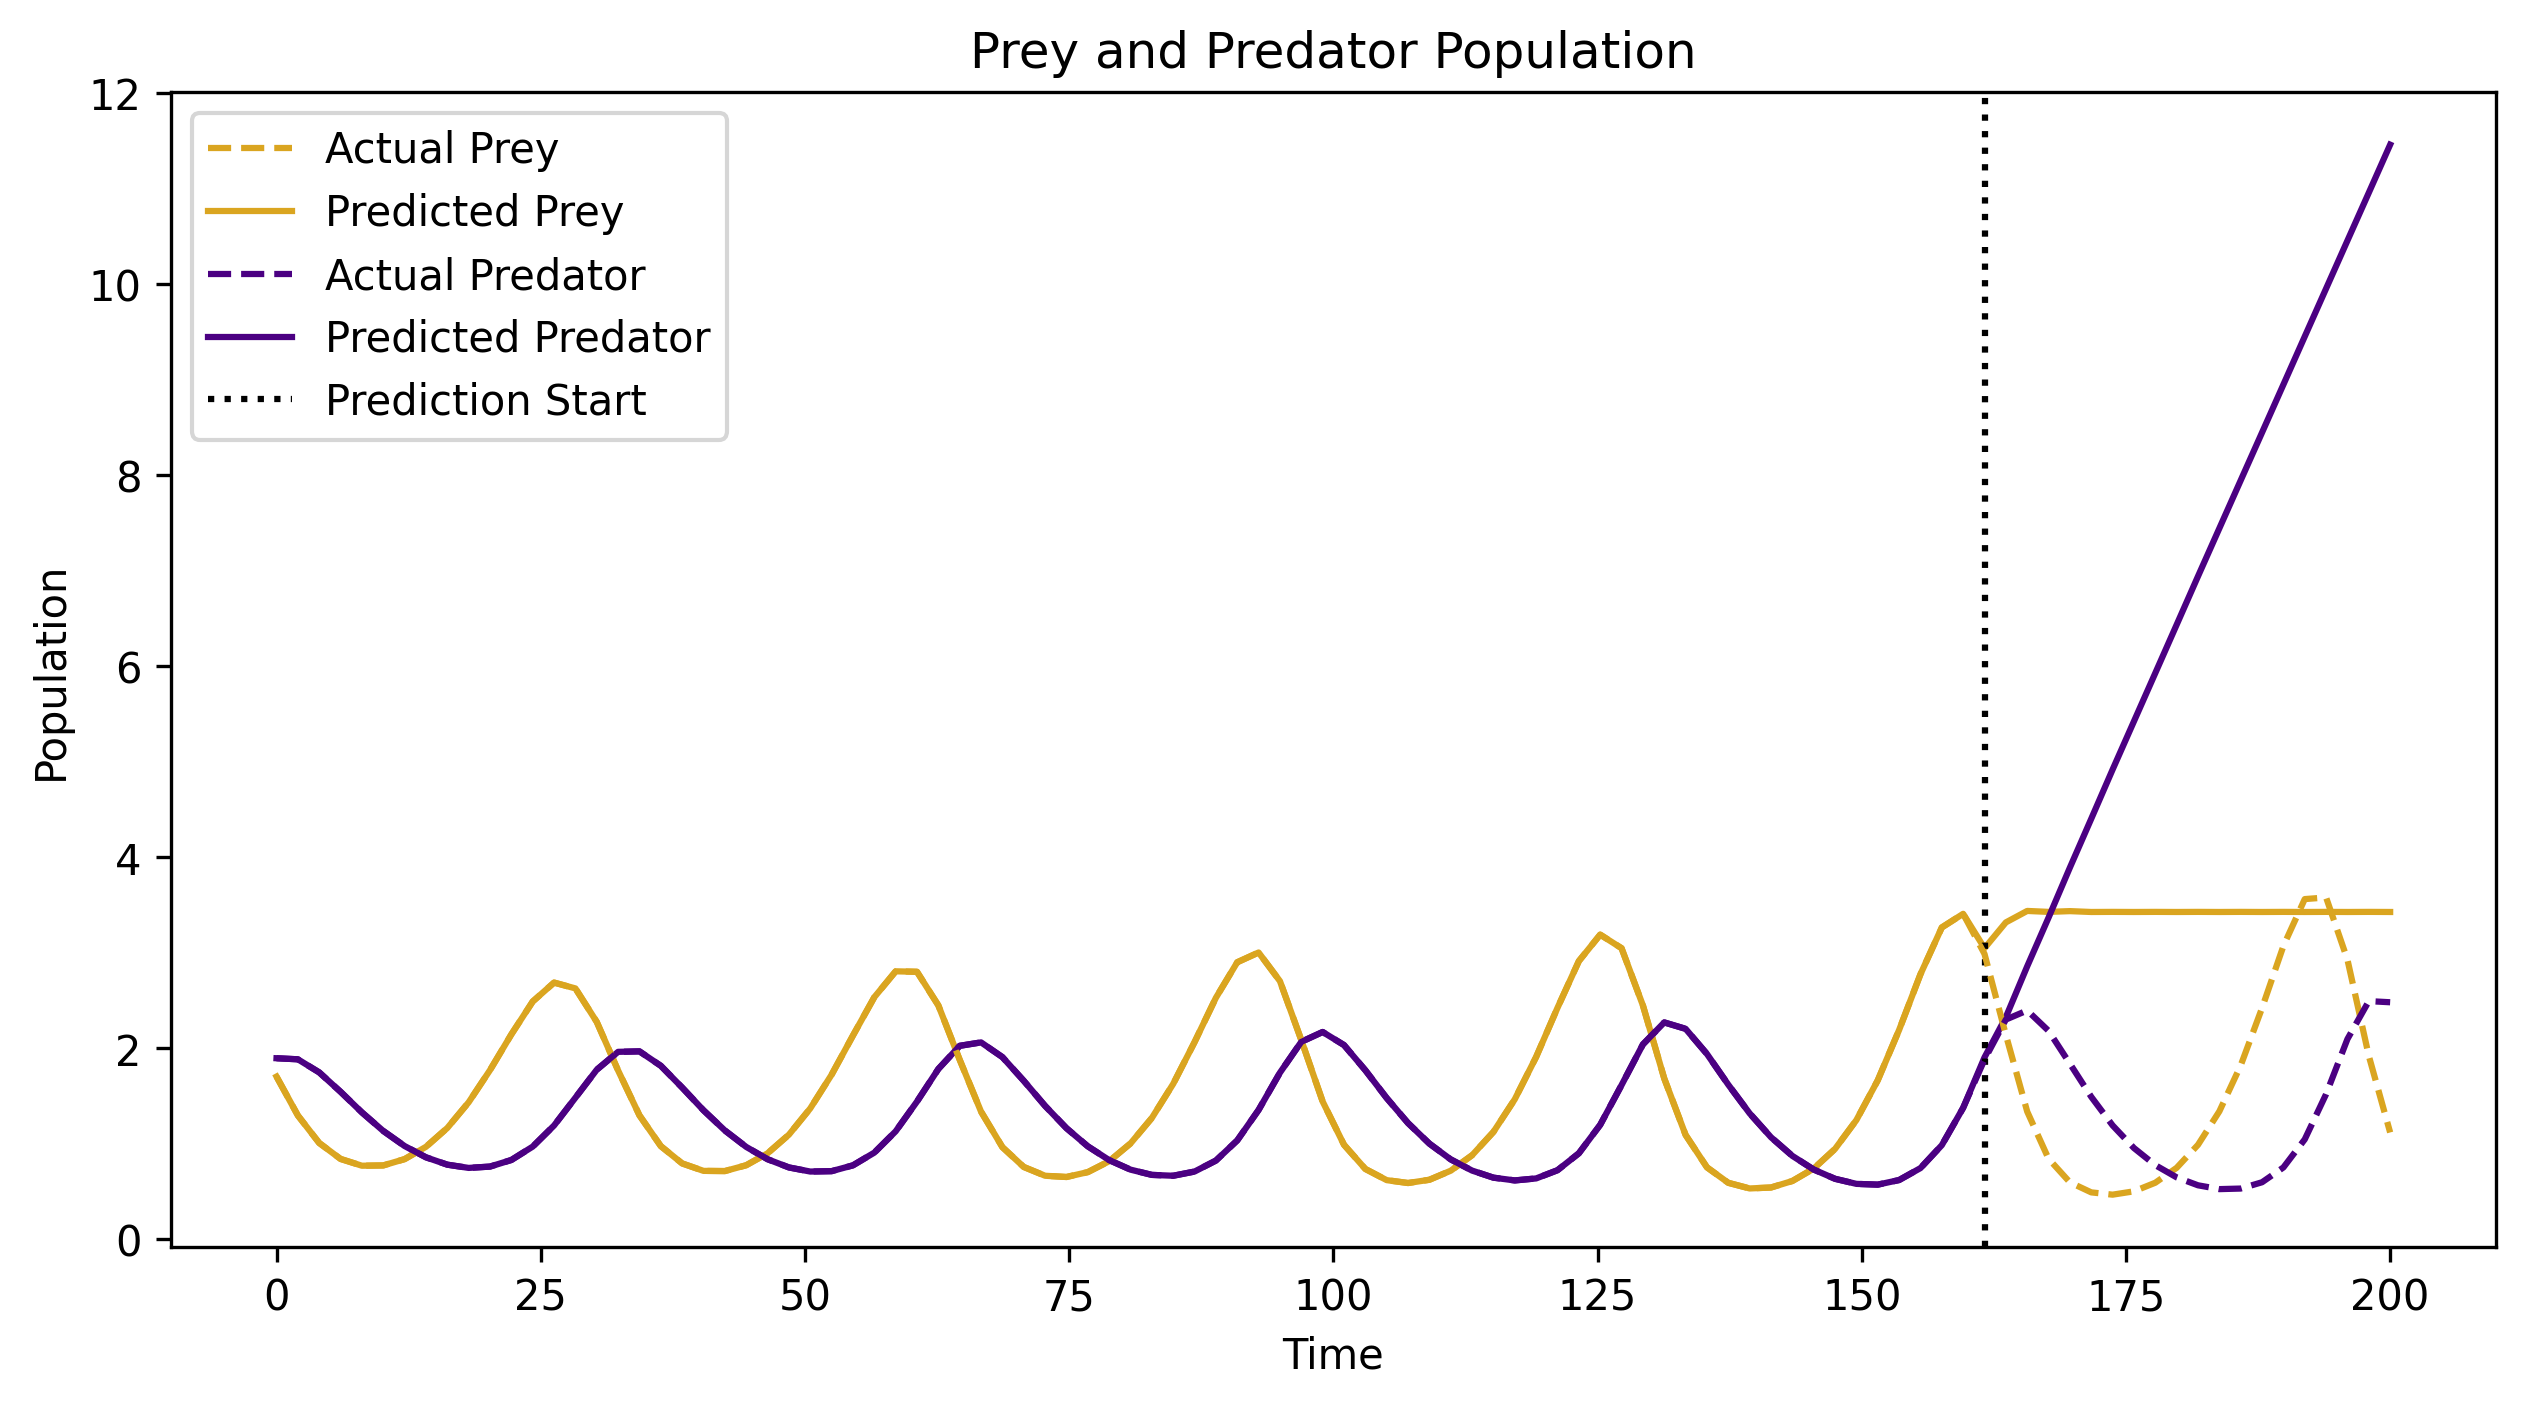
\includegraphics[width=\columnwidth, keepaspectratio]{../plots/predictions_example.png}
    \caption{Predictions (dashed) of the untrained model compared with the true (solid) values on a subset of the dataset for both predator (purple) and prey (gold).}
    \label{fig:baseline_pred}
\end{figure}

\begin{table}[h]
    \centering
    \begin{tabular}{c|c|c|c|c|c|c|c|c}
        & \multicolumn{2}{c|}{506} & \multicolumn{2}{c|}{20} & \multicolumn{2}{c|}{654} & \multicolumn{2}{|c}{906} \\
        Metric & Prey & Predator & Prey & Predator & Prey & Predator & Prey & Predator \\
        \hline
        MSE & 0.217 & 0.341 & 12.207 & 10.331 & 0.001 & 0.000 & 0.023 & 0.003 \\
        RMSE & 0.465 & 0.583 & 3.494 & 3.214 & 0.030 & 0.001 & 0.151 & 0.050 \\
        MAE & 0.372 & 0.471 & 2.385 & 2.312 & 0.028 & 0.001 & 0.103 & 0.032 \\
        MAPE & 0.301 & 0.365 & 1.332 & 0.760 & 0.004 & 0.001 & 0.031 & 0.056 \\
    \end{tabular}
    \caption{Metrics for the untrained model performance on a subset of the test set.}
    \label{tab:baseline}
\end{table}

\begin{figure}
    \centering
    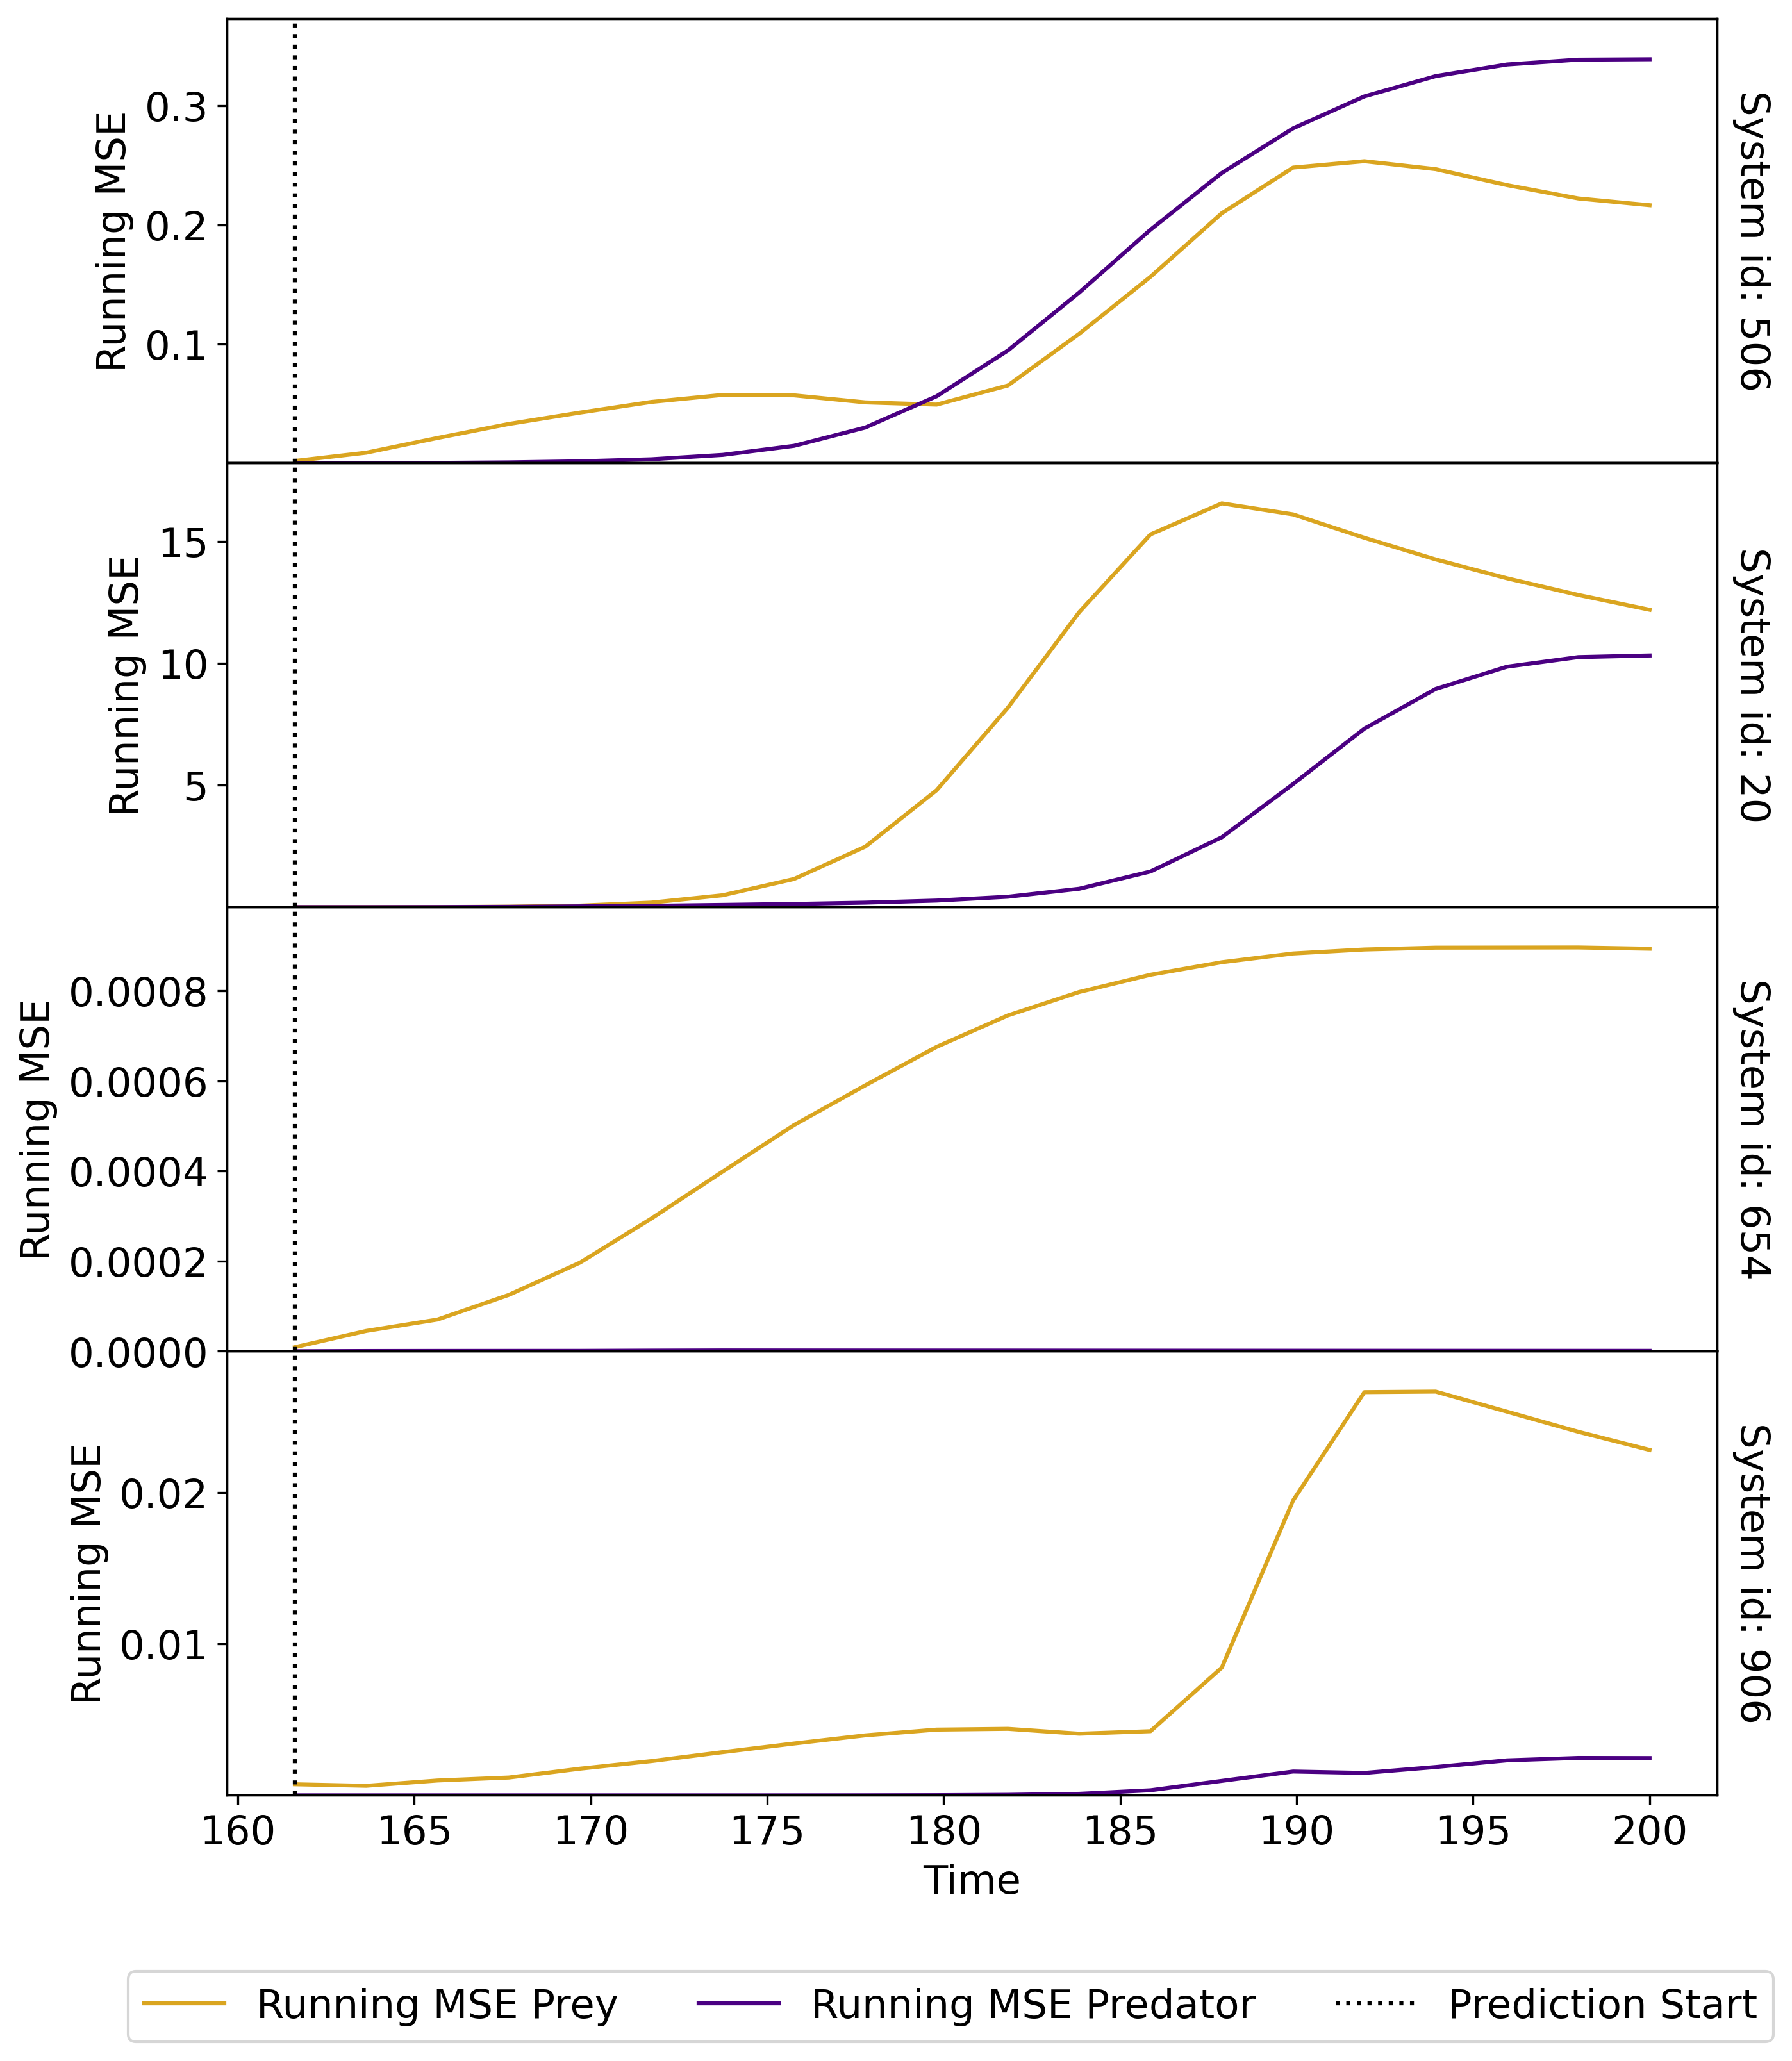
\includegraphics[width=\columnwidth, keepaspectratio]{../plots/running_mse_example.png}
    \caption{Running mean squared error (RMSE) for the model on a subset of the test set over the out-of-distribution data for the predator (purple) and prey (gold) time series.}
    \label{fig:baseline_rmse}
\end{figure}

As can be seen in Fig.~\ref{fig:baseline_pred}, the untrained model is fairly capable at predicting the oscillatory and stable systems 906 and 654 respectively, but is unable to predict decaying and growing systems 506 and 20 very well. This is reflected in the metrics shown in Table~\ref{tab:baseline}, where the error metrics for systems 654 and 906 are all very small, but the metrics for systems 506 and 20 are significantly greater. The model is especially terrible at predicting system 20, the growing system. 

What also seems important is where the model begins to forecast. This is demonstrated especially by system 654, which settled into a fairly stable and predictable state before the cut-off point, and so the model is able to predict the next 20 points very well. This is also shown by sytem 506, where the model was able to predict the rough shape of the curve, but not the exact values for the prey time series. The cut-off point occurred just after the peak of the prey time series but before the peak of the predator time series.

Without fine-tuning, it is clear that the model is unable to learn the more subtle underlying patterns in the time series data. This is probably becaues it's not been previously trained on time series forecasting tasks.
\clearpage
\section{LoRA}
\label{sec:lora}

The model was fine-tuned using the LoRA \citep{hu2021loralowrankadaptationlarge} implementation to wrap the query and value projection layers with LoRALinear layers. This adds low-rank matrices to the model's weights for the query and value matrices, which allows for efficient training and adaptation to new tasks. Then, when training the model, only the LoRA weights are updated whilst the rest of the model's weights are frozen. This allows for efficient training and adaptation to new tasks, as this approach allows for the model to be fine-tuned on a specific task without the need for retraining the entire model, which can be computationally expensive and time-consuming.

The specific parameter blocks that are being tuned when using LoRA are the A and B matrices added to the query and value projections in each transformer layer's self-attention block.

\subsection{Training with LoRA}
To demonstrate the baseline improvements when adding LoRA, the model was fine-tuned using the default hyperparameters shown in Table~\ref{tab:lora_default} for 3,000 time steps. The model was evaluated on the validation set every 50 steps. The training and validation loss are shown in Fig.~\ref{fig:lora_default_loss}, and the model's performance on stratified examples from the test set is shown in Fig.~\ref{fig:lora_default_pred}. The metrics for the model's performance on the test set are shown in Table~\ref{tab:lora_default_metrics}.

\begin{table}[h]
    \centering
    \begin{tabular}{c|c}
        Hyperparameter & Value \\
        \hline
        Learning rate & $10^{-5}$ \\
        Batch size & 4 \\
        LoRA rank & 4 \\
        LoRA scaling factor $\alpha$ & 4 \\
        Maximum context length & 512 \\
    \end{tabular}
    \caption{Default hyperparameters used for training the model with LoRA on the dataset.}
    \label{tab:lora_default}
\end{table}

\begin{figure}[h]
    \centering
    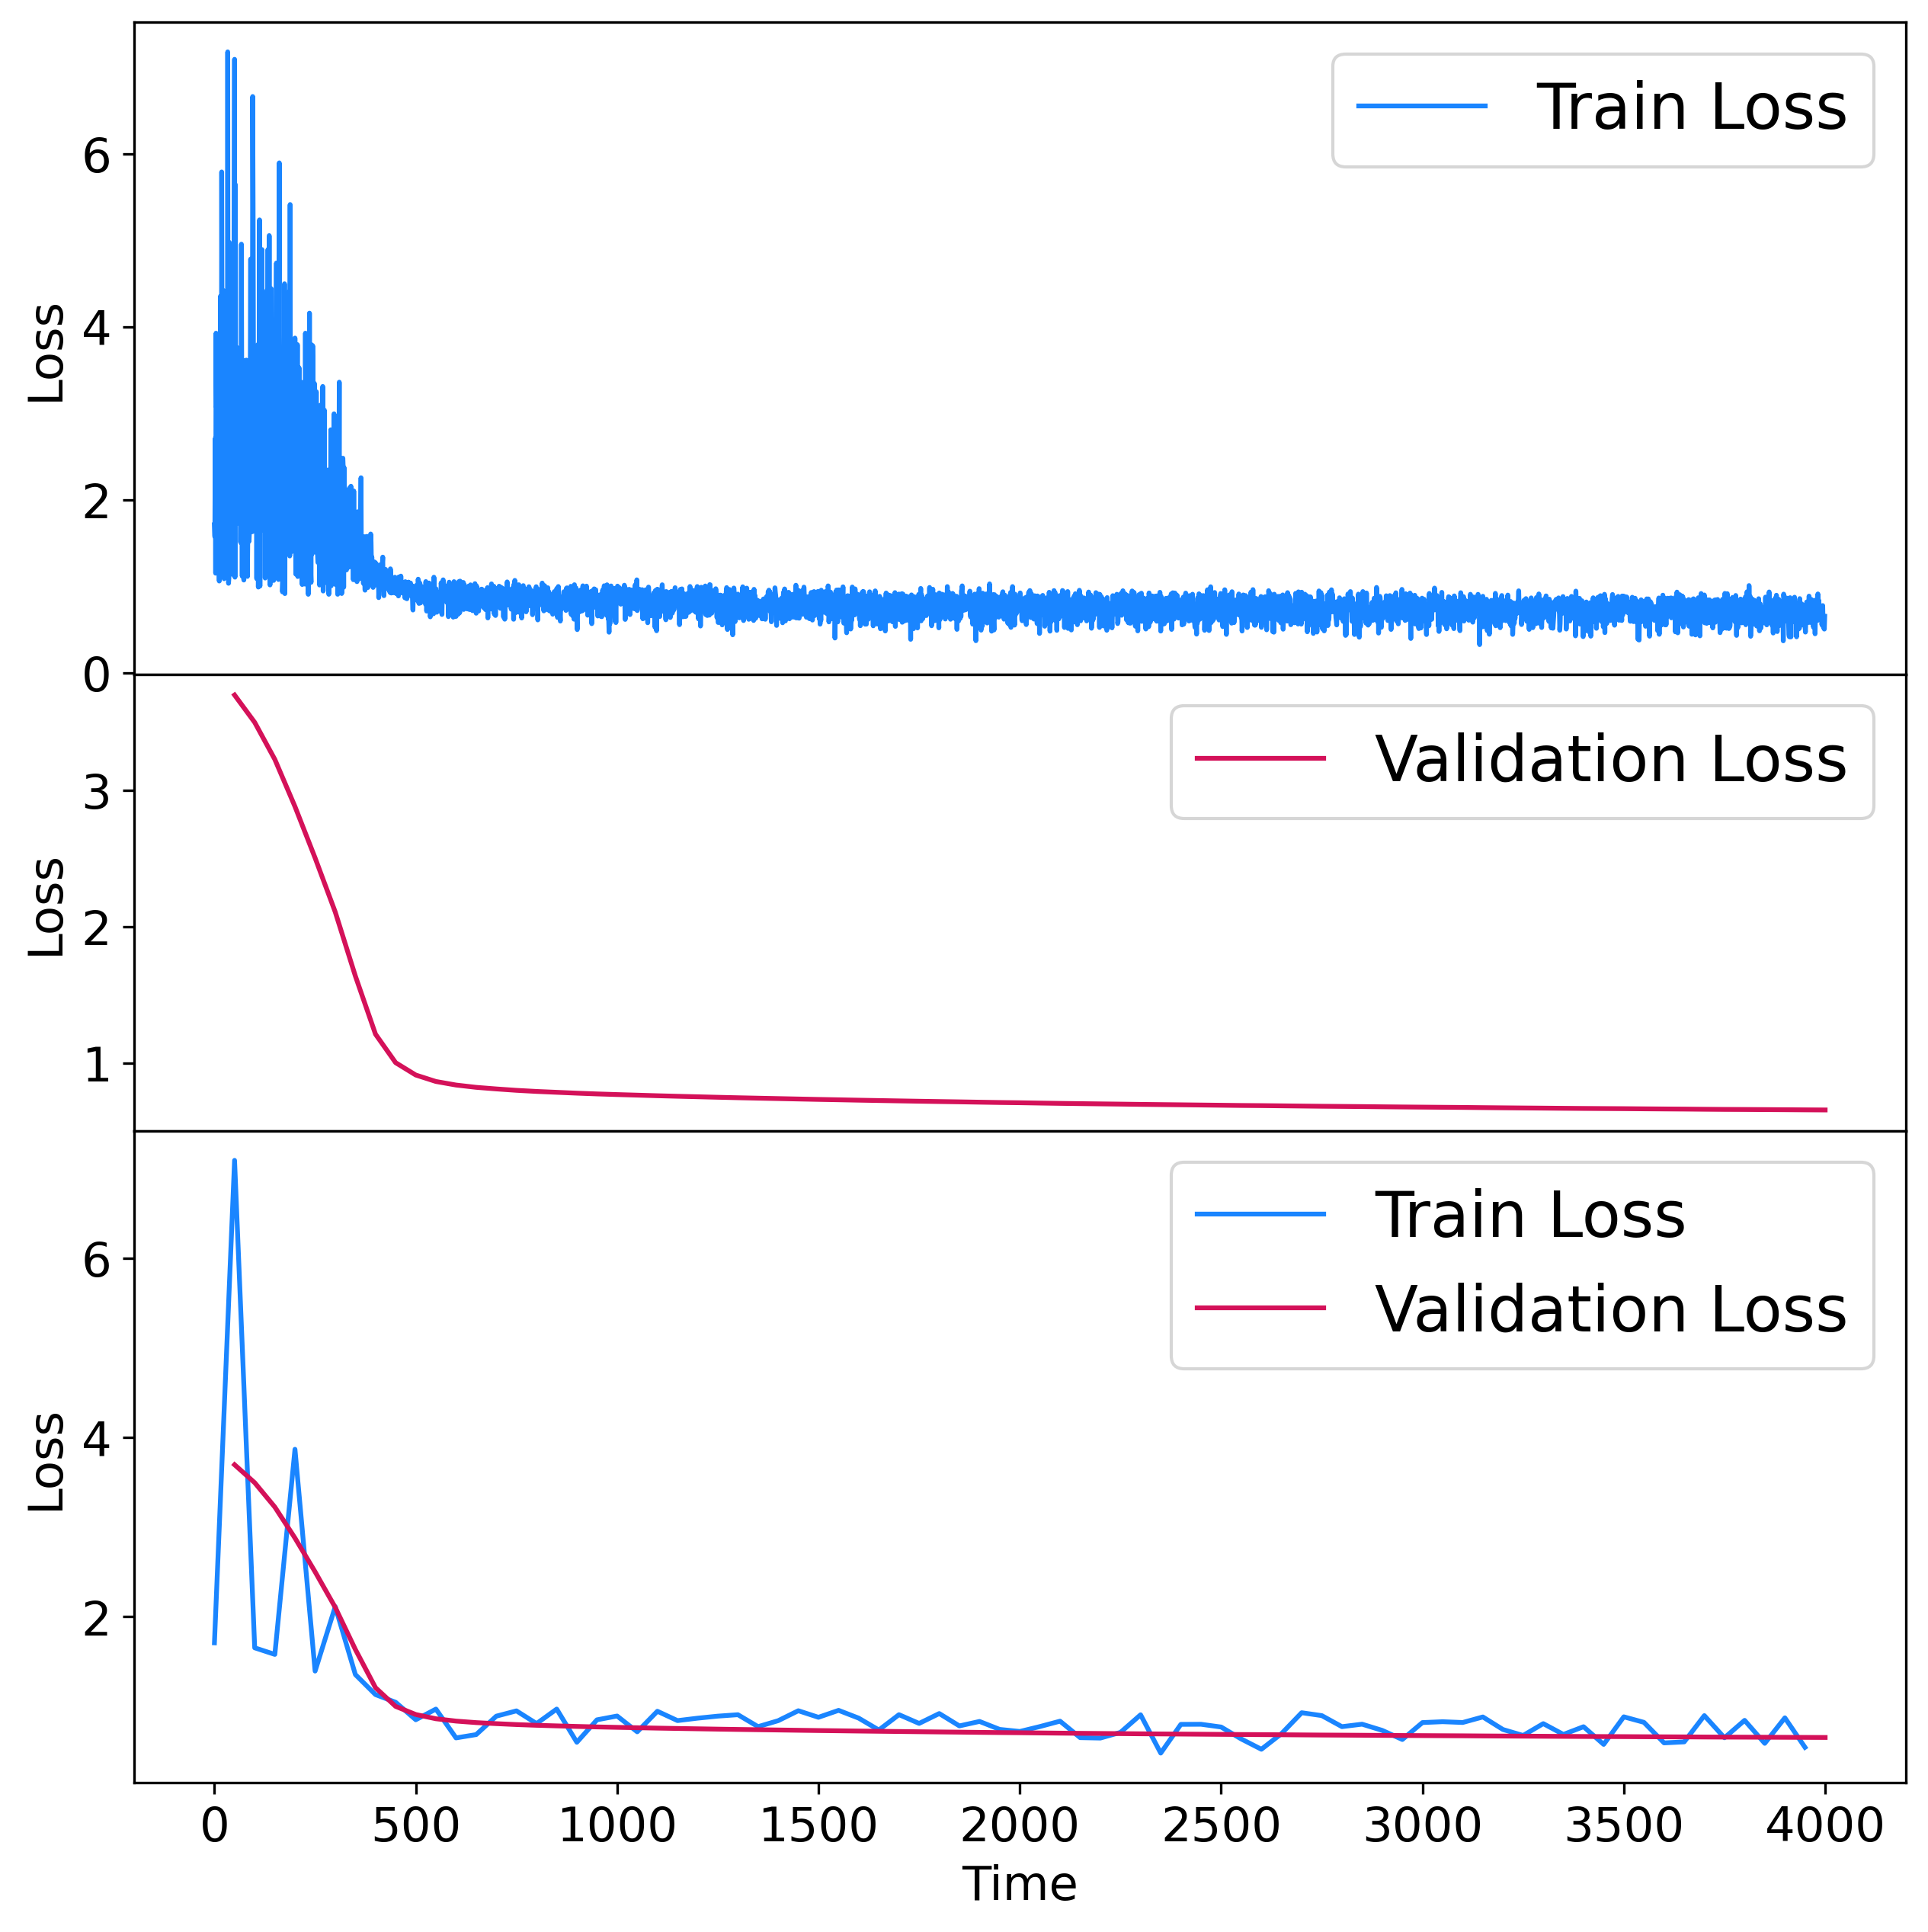
\includegraphics[width=\columnwidth, keepaspectratio]{../plots/lora_default_loss.png}
    \caption{Training and validation loss for the model fine-tuned with LoRA on the dataset using default hyperparameters. The bottom figure compares the training (blue) and validation (red) loss using the same resolution of every 50 steps.}
    \label{fig:lora_default_loss}
\end{figure}

\begin{figure}
    \centering
    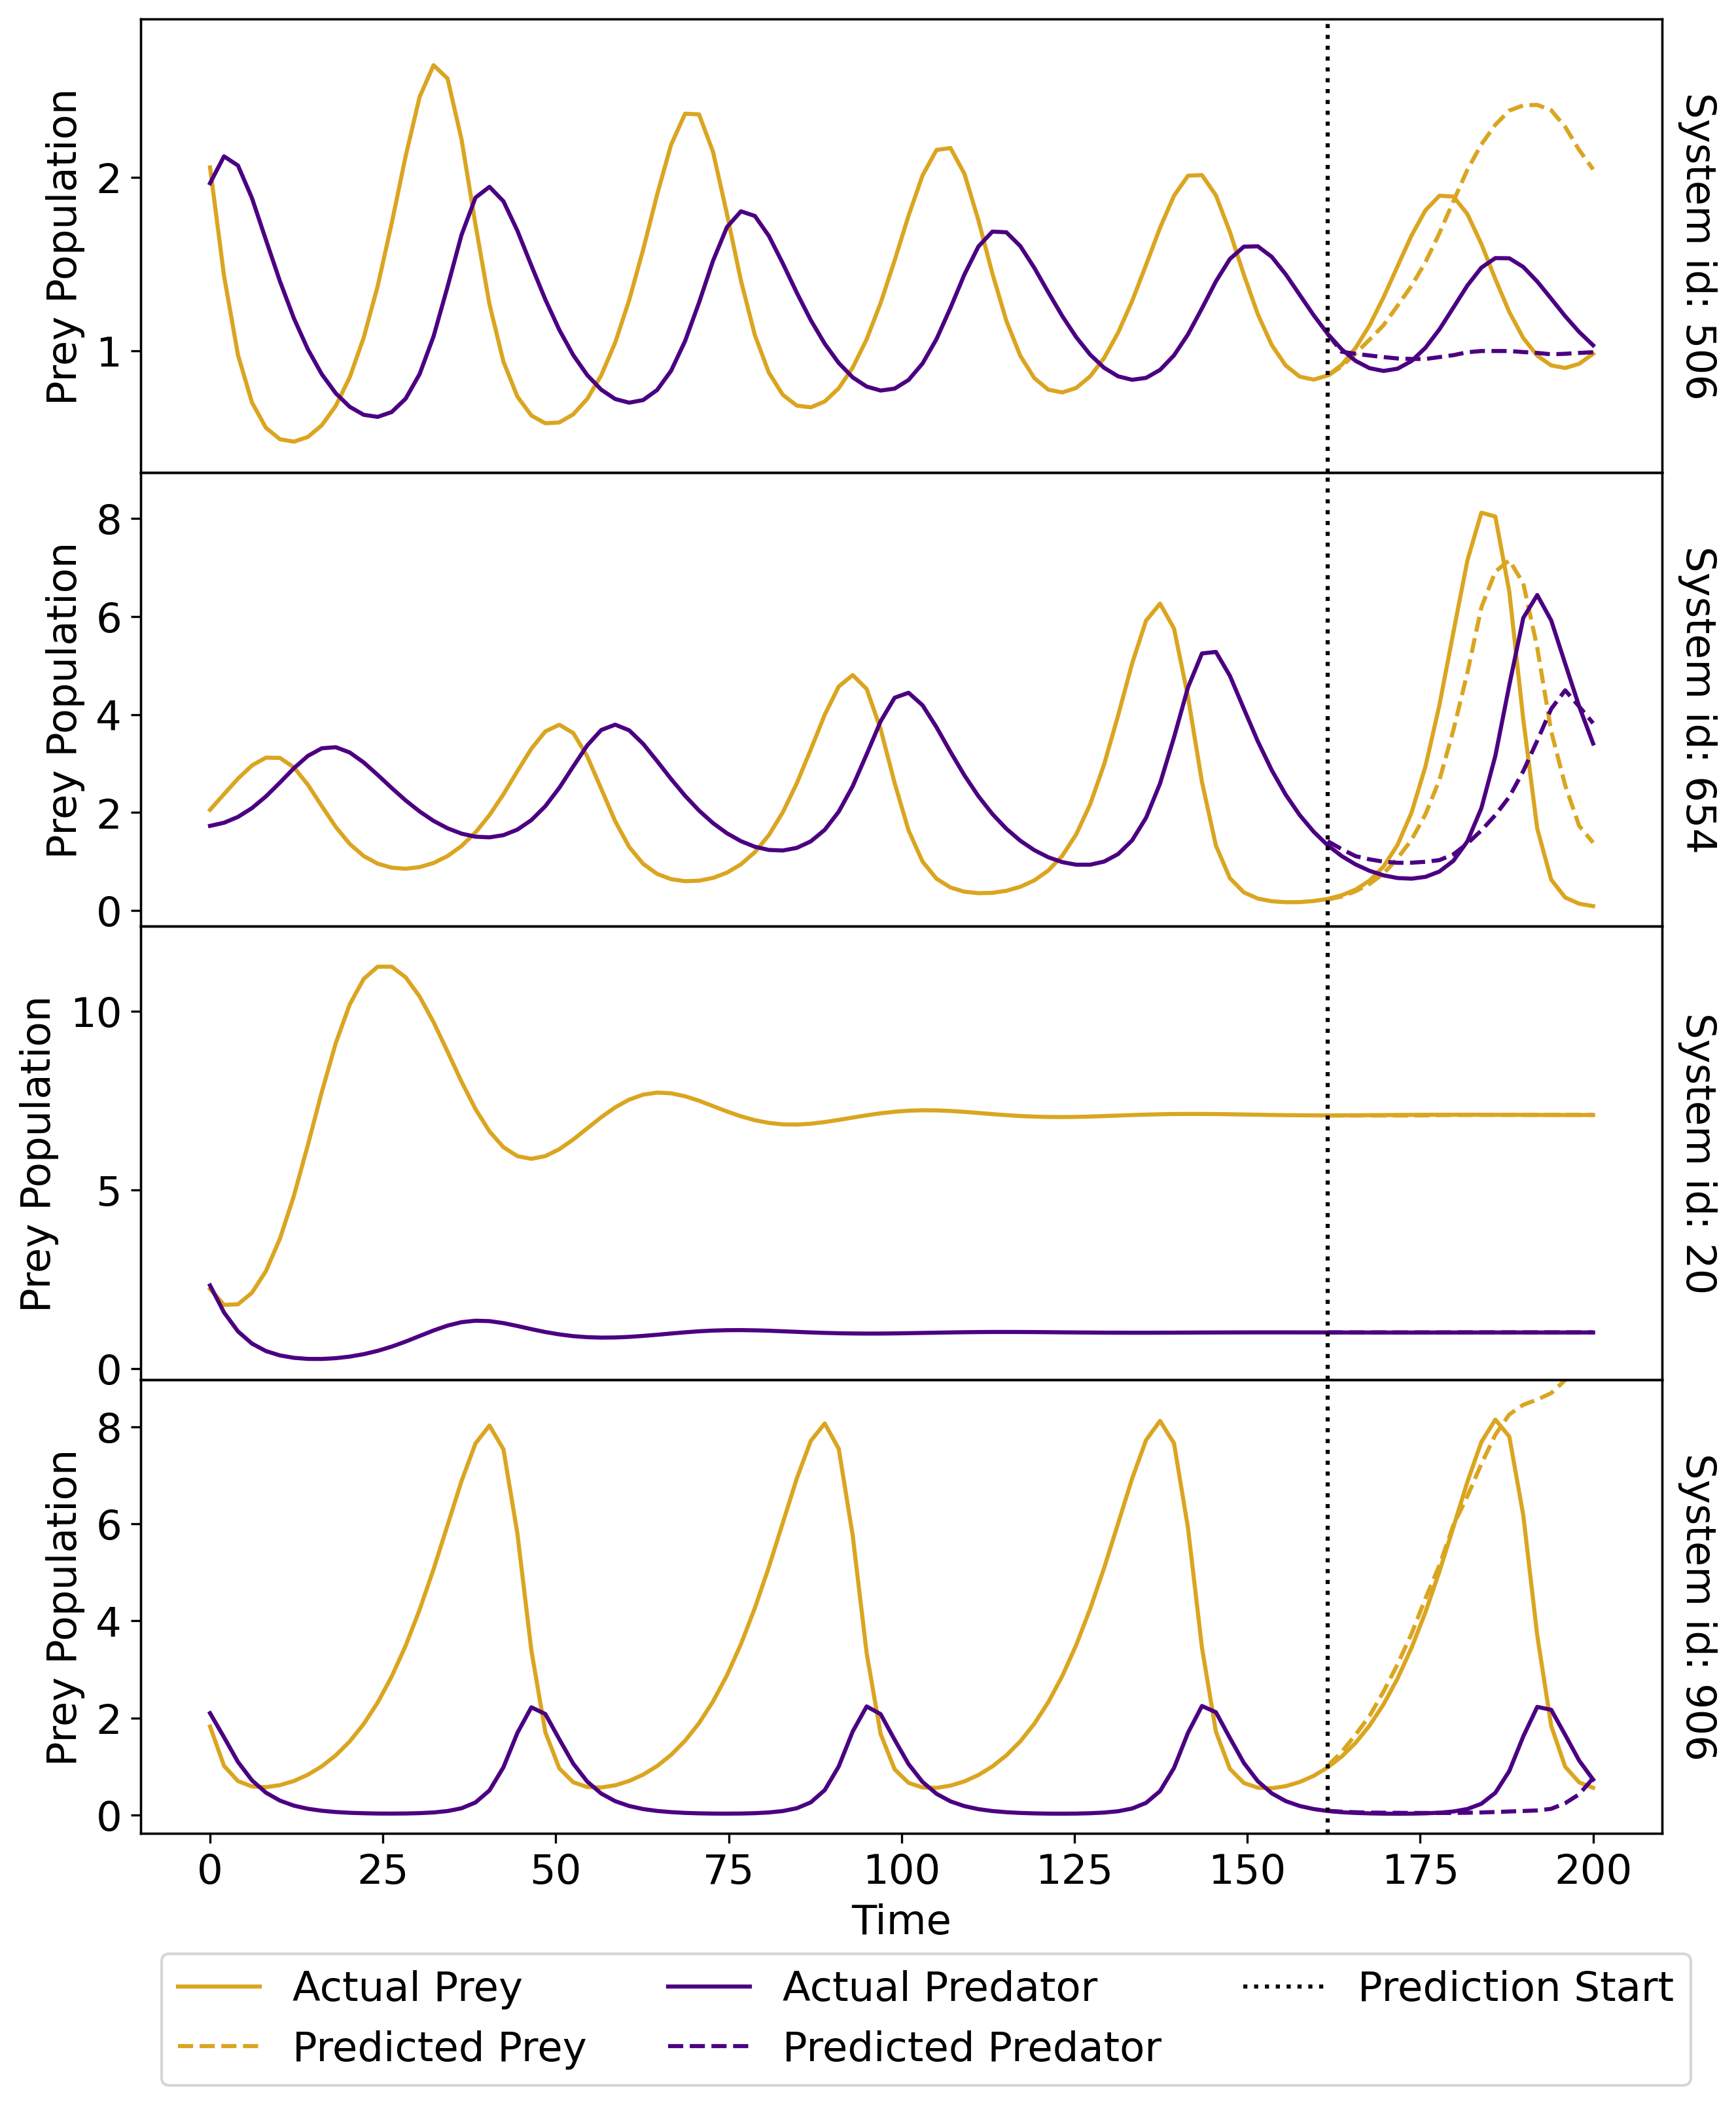
\includegraphics[width=\columnwidth, keepaspectratio]{../plots/predictions_lora_default.png}
    \caption{Predictions (dashed) of the model fine-tuned with LoRA using default hyperparameters compared with the true (solid) values on a subset of the test set for both predator (purple) and prey (gold).}
    \label{fig:lora_default_pred}
\end{figure}
\clearpage
\begin{table}
    \centering
    \begin{tabular}{c|c|c|c|c|c|c|c|c}
        & \multicolumn{2}{c|}{506} & \multicolumn{2}{c|}{20} & \multicolumn{2}{c|}{654} & \multicolumn{2}{|c}{906} \\
        Metric & Prey & Predator & Prey & Predator & Prey & Predator & Prey & Predator \\
        \hline
        MSE & 1.561 & 0.227 & 6.618 & 6.994 & 0.004 & 0.000 & 37.543 & 24.459 \\
        RMSE & 1.249 & 0.477 & 2.573 & 2.645 & 0.061 & 0.005 & 6.127 & 4.946 \\
        MAE & 0.880 & 0.388 & 1.962 & 1.775 & 0.038 & 0.005 & 3.545 & 2.393 \\
        MAPE & 0.837 & 0.300 & 4.530 & 0.493 & 0.005 & 0.005 & 3.397 & 2.592 \\
    \end{tabular}
    \caption{Metrics for the model fine-tuned with LoRA using default hyperparameters on a subset of the test set.}
    \label{tab:lora_default_metrics}
\end{table}
As can be seen in Fig.~\ref{fig:lora_default_loss}, there is a gradual plateau in the training and validation loss starting around 1,000 steps, indicating that the model is converging to a local minimum. The validation loss is comparable to the training loss but generally higher, which indicates that the model is not overfitting to the training data. 

As shown by Fig.~\ref{fig:lora_default_pred}, the model performs somewhat better on predicting the growing and decaying systems, as it seems to understand that there is an underlying pattern of growing or decaying oscillations. However, it now struggles with the oscillatory system 906, which now has fairly large errors in both the prey and predator time series predictions. This is very different to before, where it was able to predict it almost perfectly, as seen in Figures~\ref{fig:baseline_pred} and \ref{fig:baseline_rmse}. This is likely because very few oscillatory systems are present in the entire Lotka-Volterra dataset, with most of the systems being some form of decaying or growing.

The gradients of the A and B matrices were tracked throughout the training process and it was found that the gradients of the A and B matrices neither exploded nor vanished. Thus, gradient clipping was not applied to the model. As the figure is quite large, comprising of 48 plots, it is not shown in this report and is instead included as supplementary material in the \texttt{addendum} folder.

\subsection{Hyperparameter tuning}
To further improve the performance of the model fine-tuned with LoRA, hyperparameter tuning was performed. The hyperparameters that were tuned are shown in Table~\ref{tab:lora_tuning}. They were tuned using a grid search approach, and the best combination of hyperparameters was then selected based on the final validation loss.

\begin{table}
    \centering
    \begin{tabular}{c|c}
        Hyperparameter & Values \\
        \hline
        Learning rate & $10^{-5}$, $5\times10^{-5}$, $10^{-5}$ \\
        LoRA rank & 2, 4, 8 \\
        Maximum context length & 128, 512, 768 \\
    \end{tabular}
    \caption{Hyperparameters tuned for the model fine-tuned with LoRA on the dataset.}
    \label{tab:lora_tuning}
\end{table}

\subsubsection{Learning rate and LoRA rank}
\label{sec:lora_lr}
The learning rate $\eta$ and LoRA rank $r$ were tuned first, with the maximum context length set to 512. The model was trained for 300 steps with each combination of hyperparameters. The training and validation loss are shown in Fig.~\ref{fig:lora_lr_rank_loss}.

\begin{figure}
    \centering
    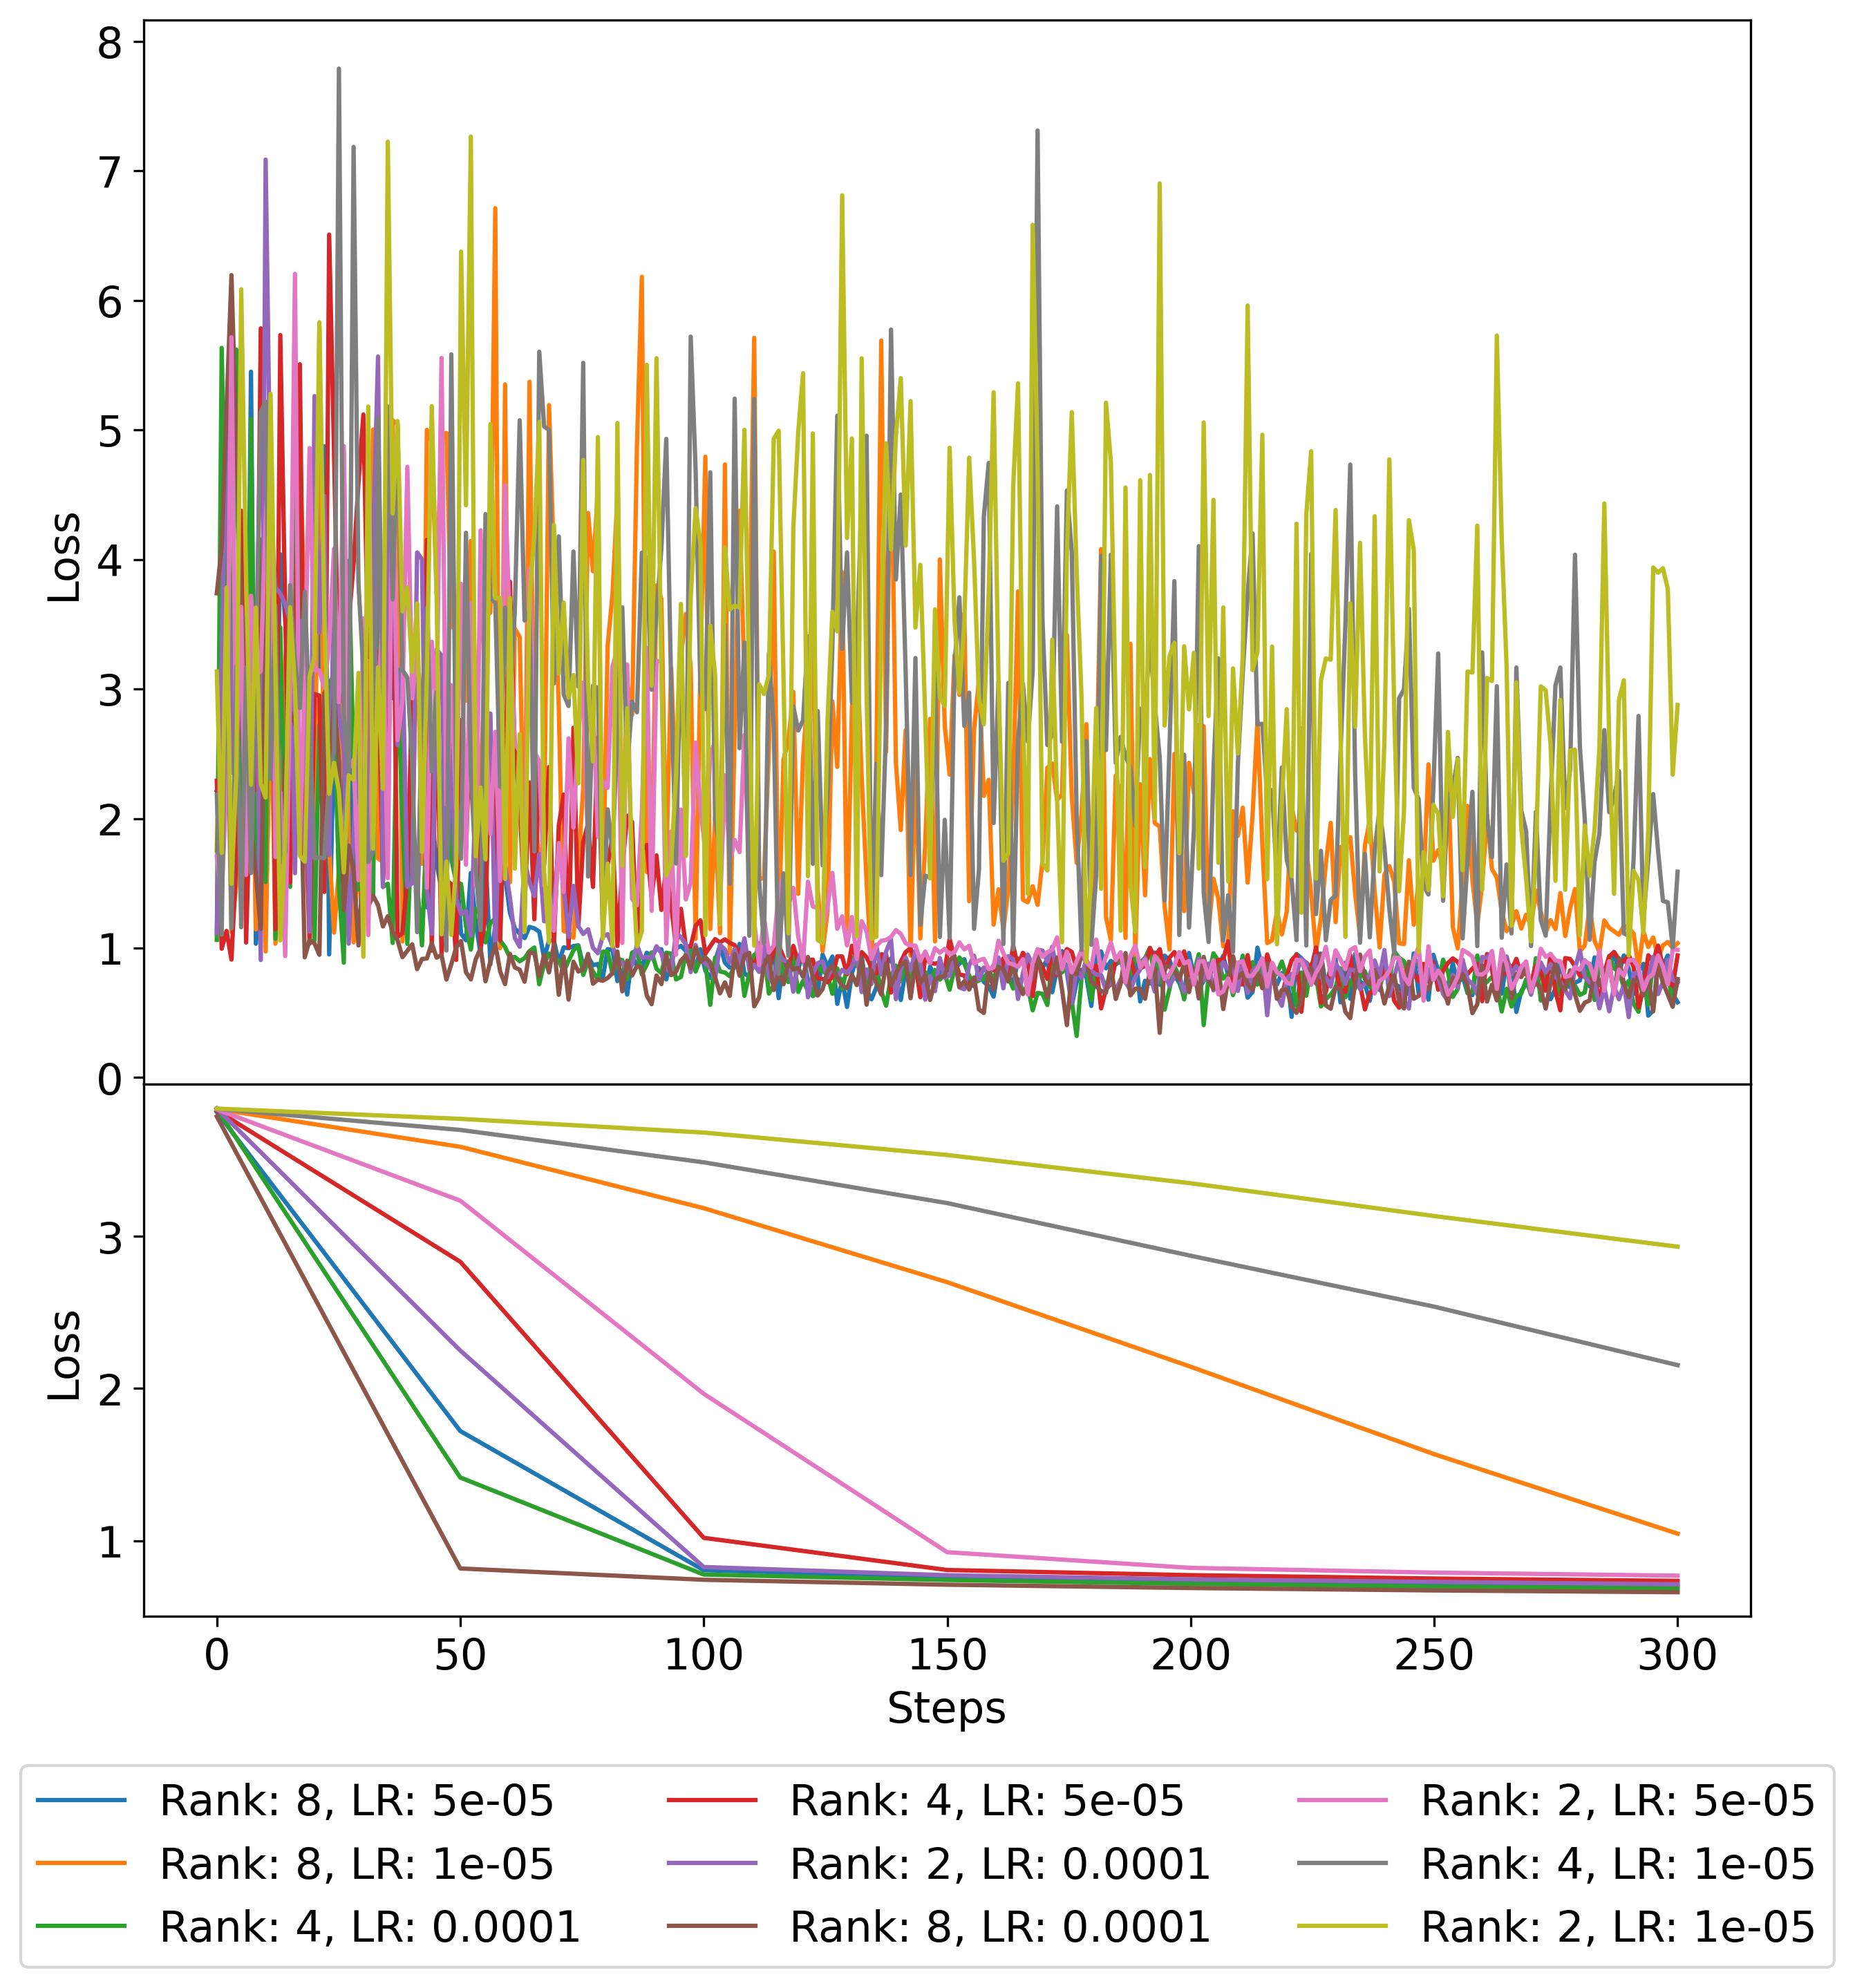
\includegraphics[width=\columnwidth, keepaspectratio]{../plots/lora_lr_rank_loss.png}
    \caption{Training (top) and validation (bottom) loss for the model fine-tuned with LoRA on the dataset using different $\eta$ and $r$.}
    \label{fig:lora_lr_rank_loss}
\end{figure}

As can be seen in Fig.~\ref{fig:lora_lr_rank_loss}, $\eta$ is has a significant impact on the model's training, with the largest learning rate $\eta=0.0001$ causing significant decreases in both training and validation loss in in the first 100 steps regardless of $r$. This is likely because with a larger $\eta$, the model is able to make large initial updates to the weights, allowing it to learn quickly from the data. However, this can also lead to instability in the training process, as the model may overshoot. Fig.~\ref{fig:lora_lr_rank_loss} also shows that $r$ also has a significant impact. As the LoRA weights are the only weights being updated, the larger the contribution the LoRA matrices are allowed to make to the model's output, the better the model is able to learn to learn from the data.

The final validation loss for each of the combinations of hyperparameters is shown in Table~\ref{tab:lora_lr_rank}. From this it can be seen that the best combination of hyperparameters is be $\eta = 10^{-4}$ and $r=8$.

\begin{table}
    \centering
    \begin{tabular}{c|c|c|c}
        Learning rate & \multicolumn{3}{|c}{LoRA Rank} \\
        & 2 & 4 & 8 \\
        \hline
        $1 \times 10^{-5}$ & 2.932 & 2.154 & 1.046 \\
        $5 \times 10^{-5}$ & 0.770 & 0.736 & 0.706 \\
        $1 \times 10^{-4}$ & 0.713 & 0.686 & 0.661 \\
    \end{tabular}
    \caption{Final validation loss for the model fine-tuned with LoRA on the dataset using different combinations of $\eta$ and $r$.}
    \label{tab:lora_lr_rank}
\end{table}
\clearpage
\subsubsection{Maximum context length}
\label{sec:max_ctx}
The maximum context length was then tuned, setting $\eta = 10^{-4}$ and $r=8$. The model was trained for 300 steps with each context length. The training and validation loss are shown in Fig.~\ref{fig:lora_max_context_loss}. 

\begin{figure}
    \centering
    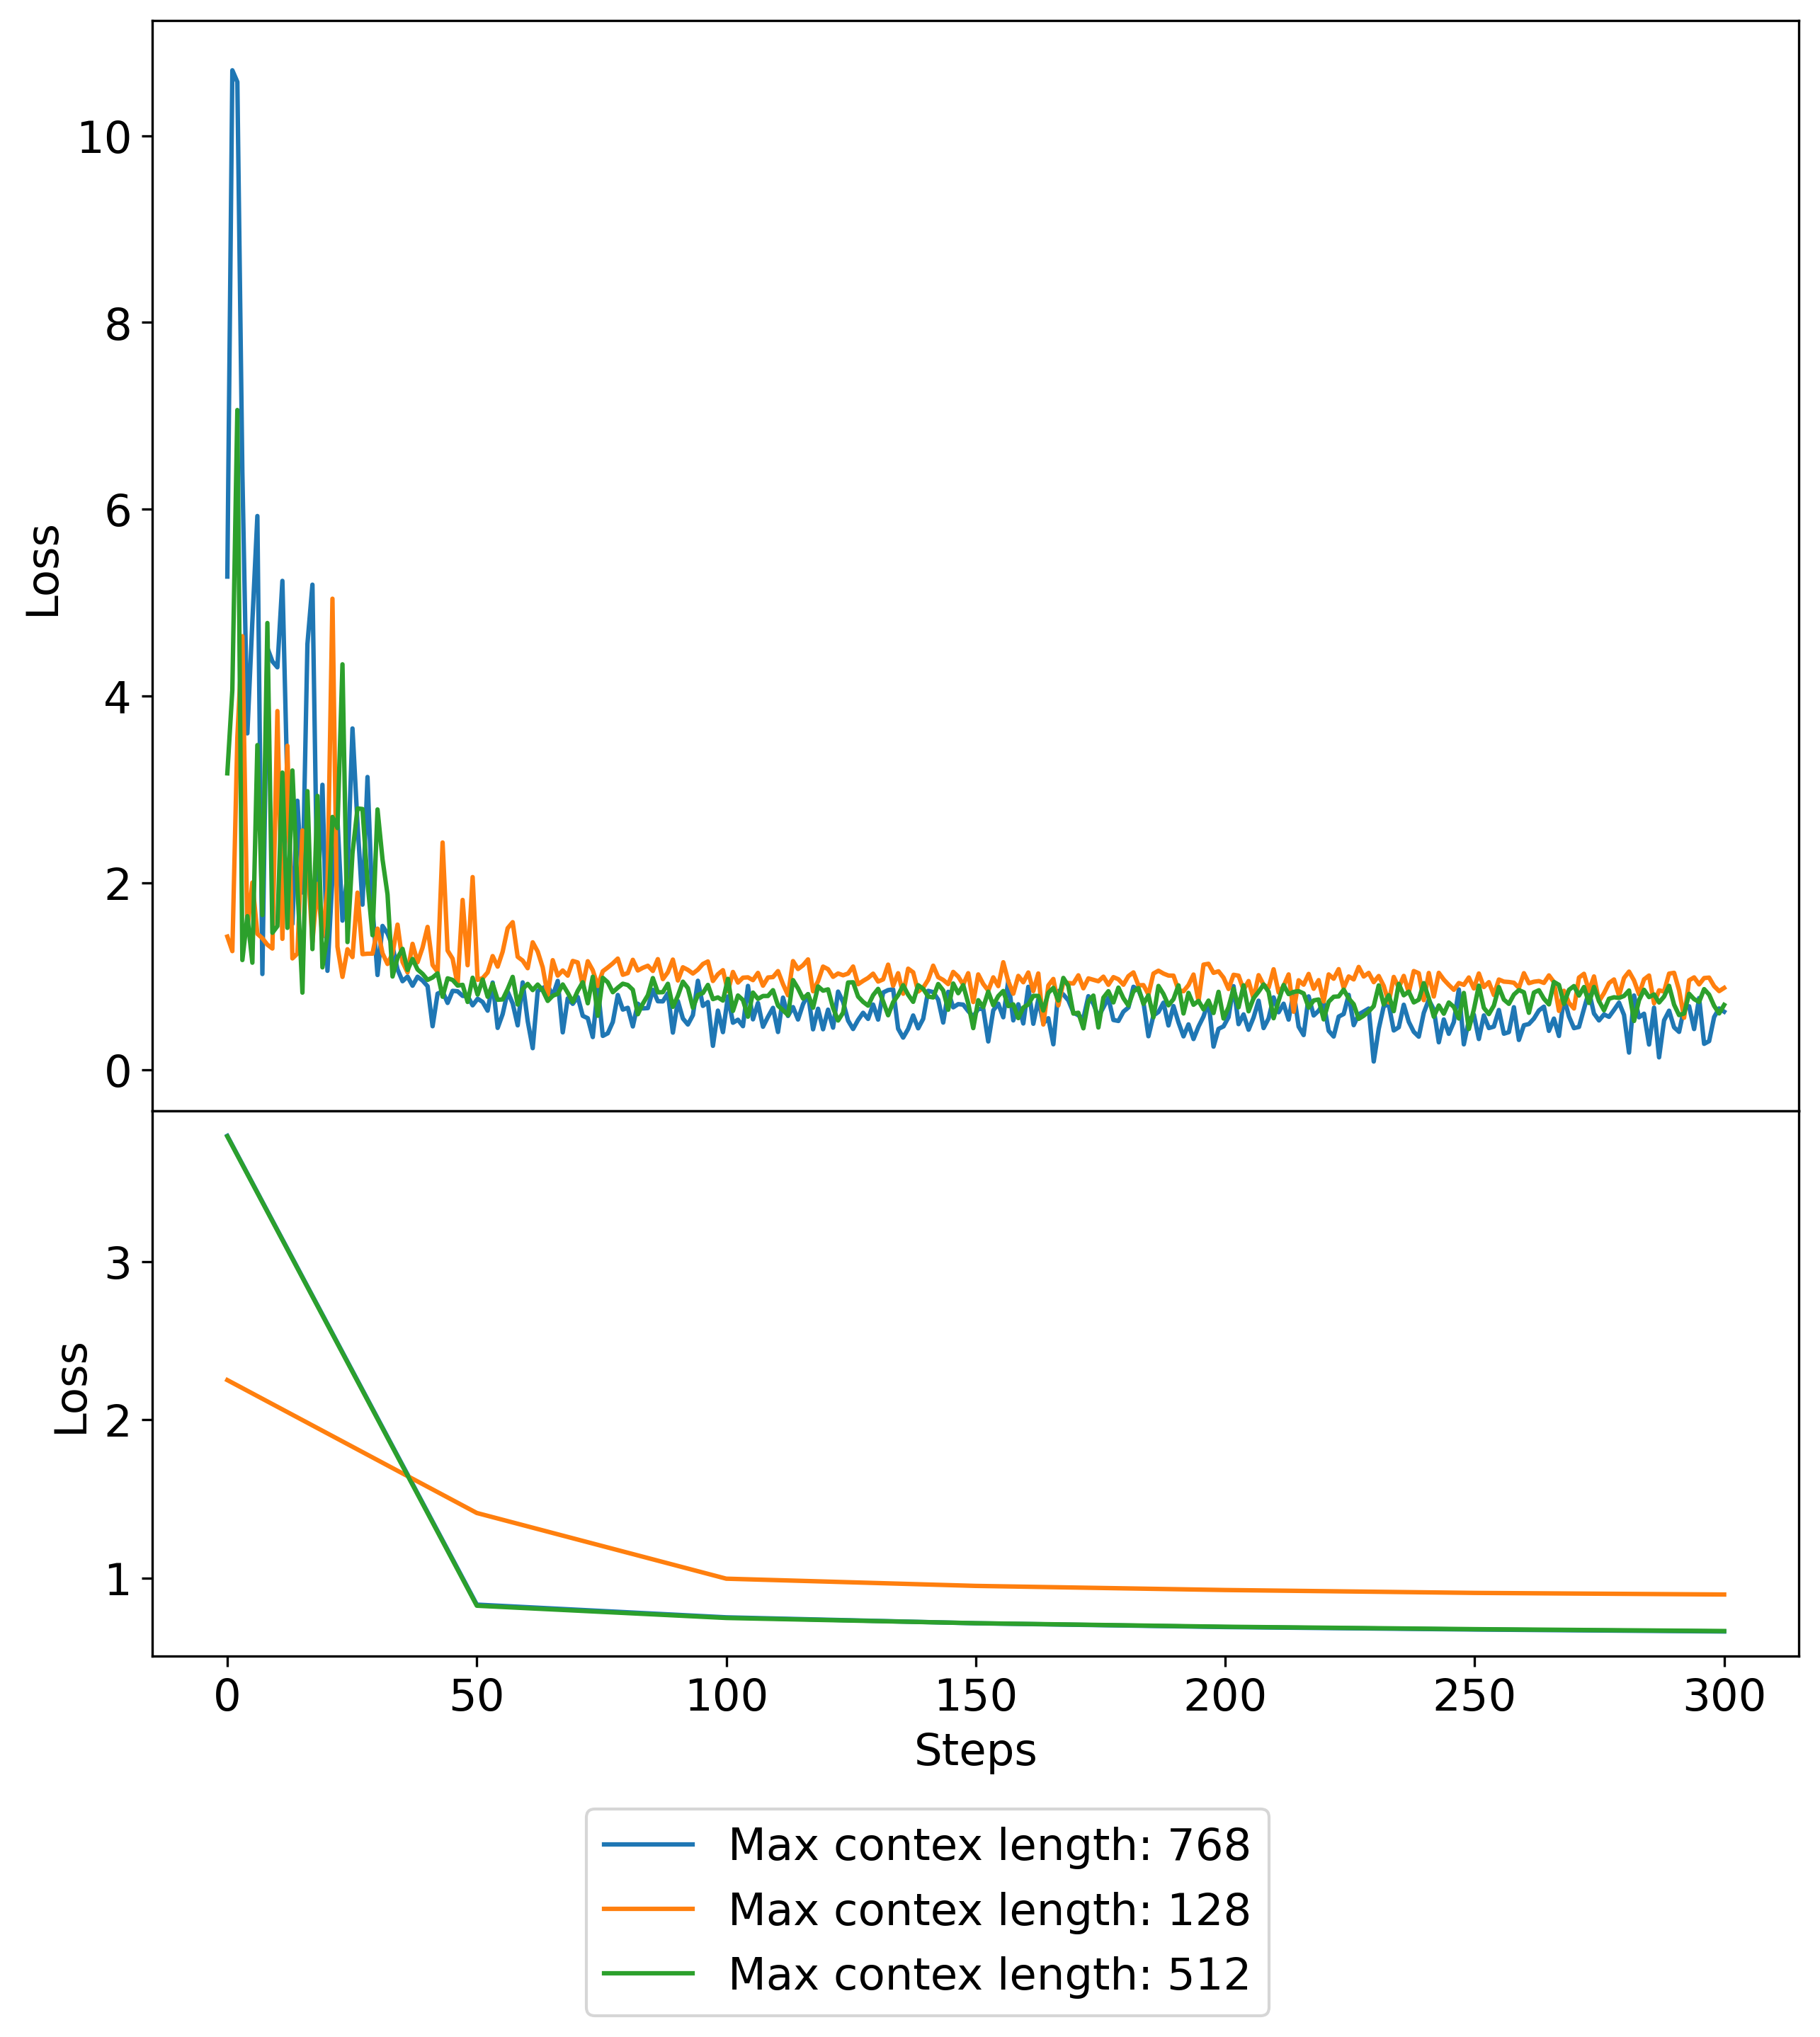
\includegraphics[width=\columnwidth, keepaspectratio]{../plots/lora_ctx_loss.png}
    \caption{Training (top) and validation (bottom) loss for the model fine-tuned with LoRA on the dataset using different maximum context lengths with $\eta=0.0001$ and $r=8$.}
    \label{fig:lora_max_context_loss}
\end{figure}

As can be seen in Fig.~\ref{fig:lora_max_context_loss}, the context length has an impact on the model's performance up to a point. With a too-small context length, the model is unable to effectively learn from the data, as it is only able to see a small portion of the time series data at any one time. However, the validation loss of the model using a length of 512 is very similar to that of a length of 768, indicating that the model is able to learn from the data effectively with either maximum context length. This is also shown in Table~\ref{tab:lora_max_context}: the longest maximum context length of 768 results in the lowest final validation loss, but not significantly lower than using 512. The training loss shown in Fig.~\ref{fig:lora_max_context_loss} also shows this.

The experiments were only run for a maximum of 300 steps as the model's training and validation loss tends to plateau at around 50--100 steps.

\begin{table}[h]
    \centering
    \begin{tabular}{c|c|c|c}
        & \multicolumn{3}{|c}{Maximum Context Length} \\
        & 128 & 512 & 768 \\
        \hline
        Validation loss & 0.895 & 0.664 & 0.661 \\
    \end{tabular}
    \caption{Final validation loss for the model fine-tuned with LoRA on the dataset using different maximum context lengths with $\eta=0.0001$ and $r=8$.}
    \label{tab:lora_max_context}
\end{table}

\clearpage
\subsection{Final model}
\label{sec:final_model}
Using the final hyperparameters, shown in Table~\ref{tab:lora_final_hyperparameters}, the model was fine-tuned on the dataset for 15,000 steps. The training and validation loss are shown in Fig.~\ref{fig:lora_final_loss}, and the model's performance on stratified examples from the test set is shown in Fig.~\ref{fig:lora_final_pred}. The metrics for the model's performance on a selected stratified subset of test set are shown in Table~\ref{tab:lora_final_metrics}. The running MSE for the subset is shown in Fig.~\ref{fig:lora_final_rmse}.

\begin{table}[h]
    \centering
    \begin{tabular}{c|c}
        Hyperparameter & Value \\
        \hline
        Learning rate & $10^{-4}$ \\
        LoRA rank & 8 \\
        Maximum context length & 768 \\
        Batch size & 4 \\
        LoRA scaling factor $\alpha$ & 8 \\
    \end{tabular}
    \caption{Final best hyperparameters for the model fine-tuned with LoRA on the dataset.}\label{tab:lora_final_hyperparameters}
\end{table}

\begin{figure}
    \centering
    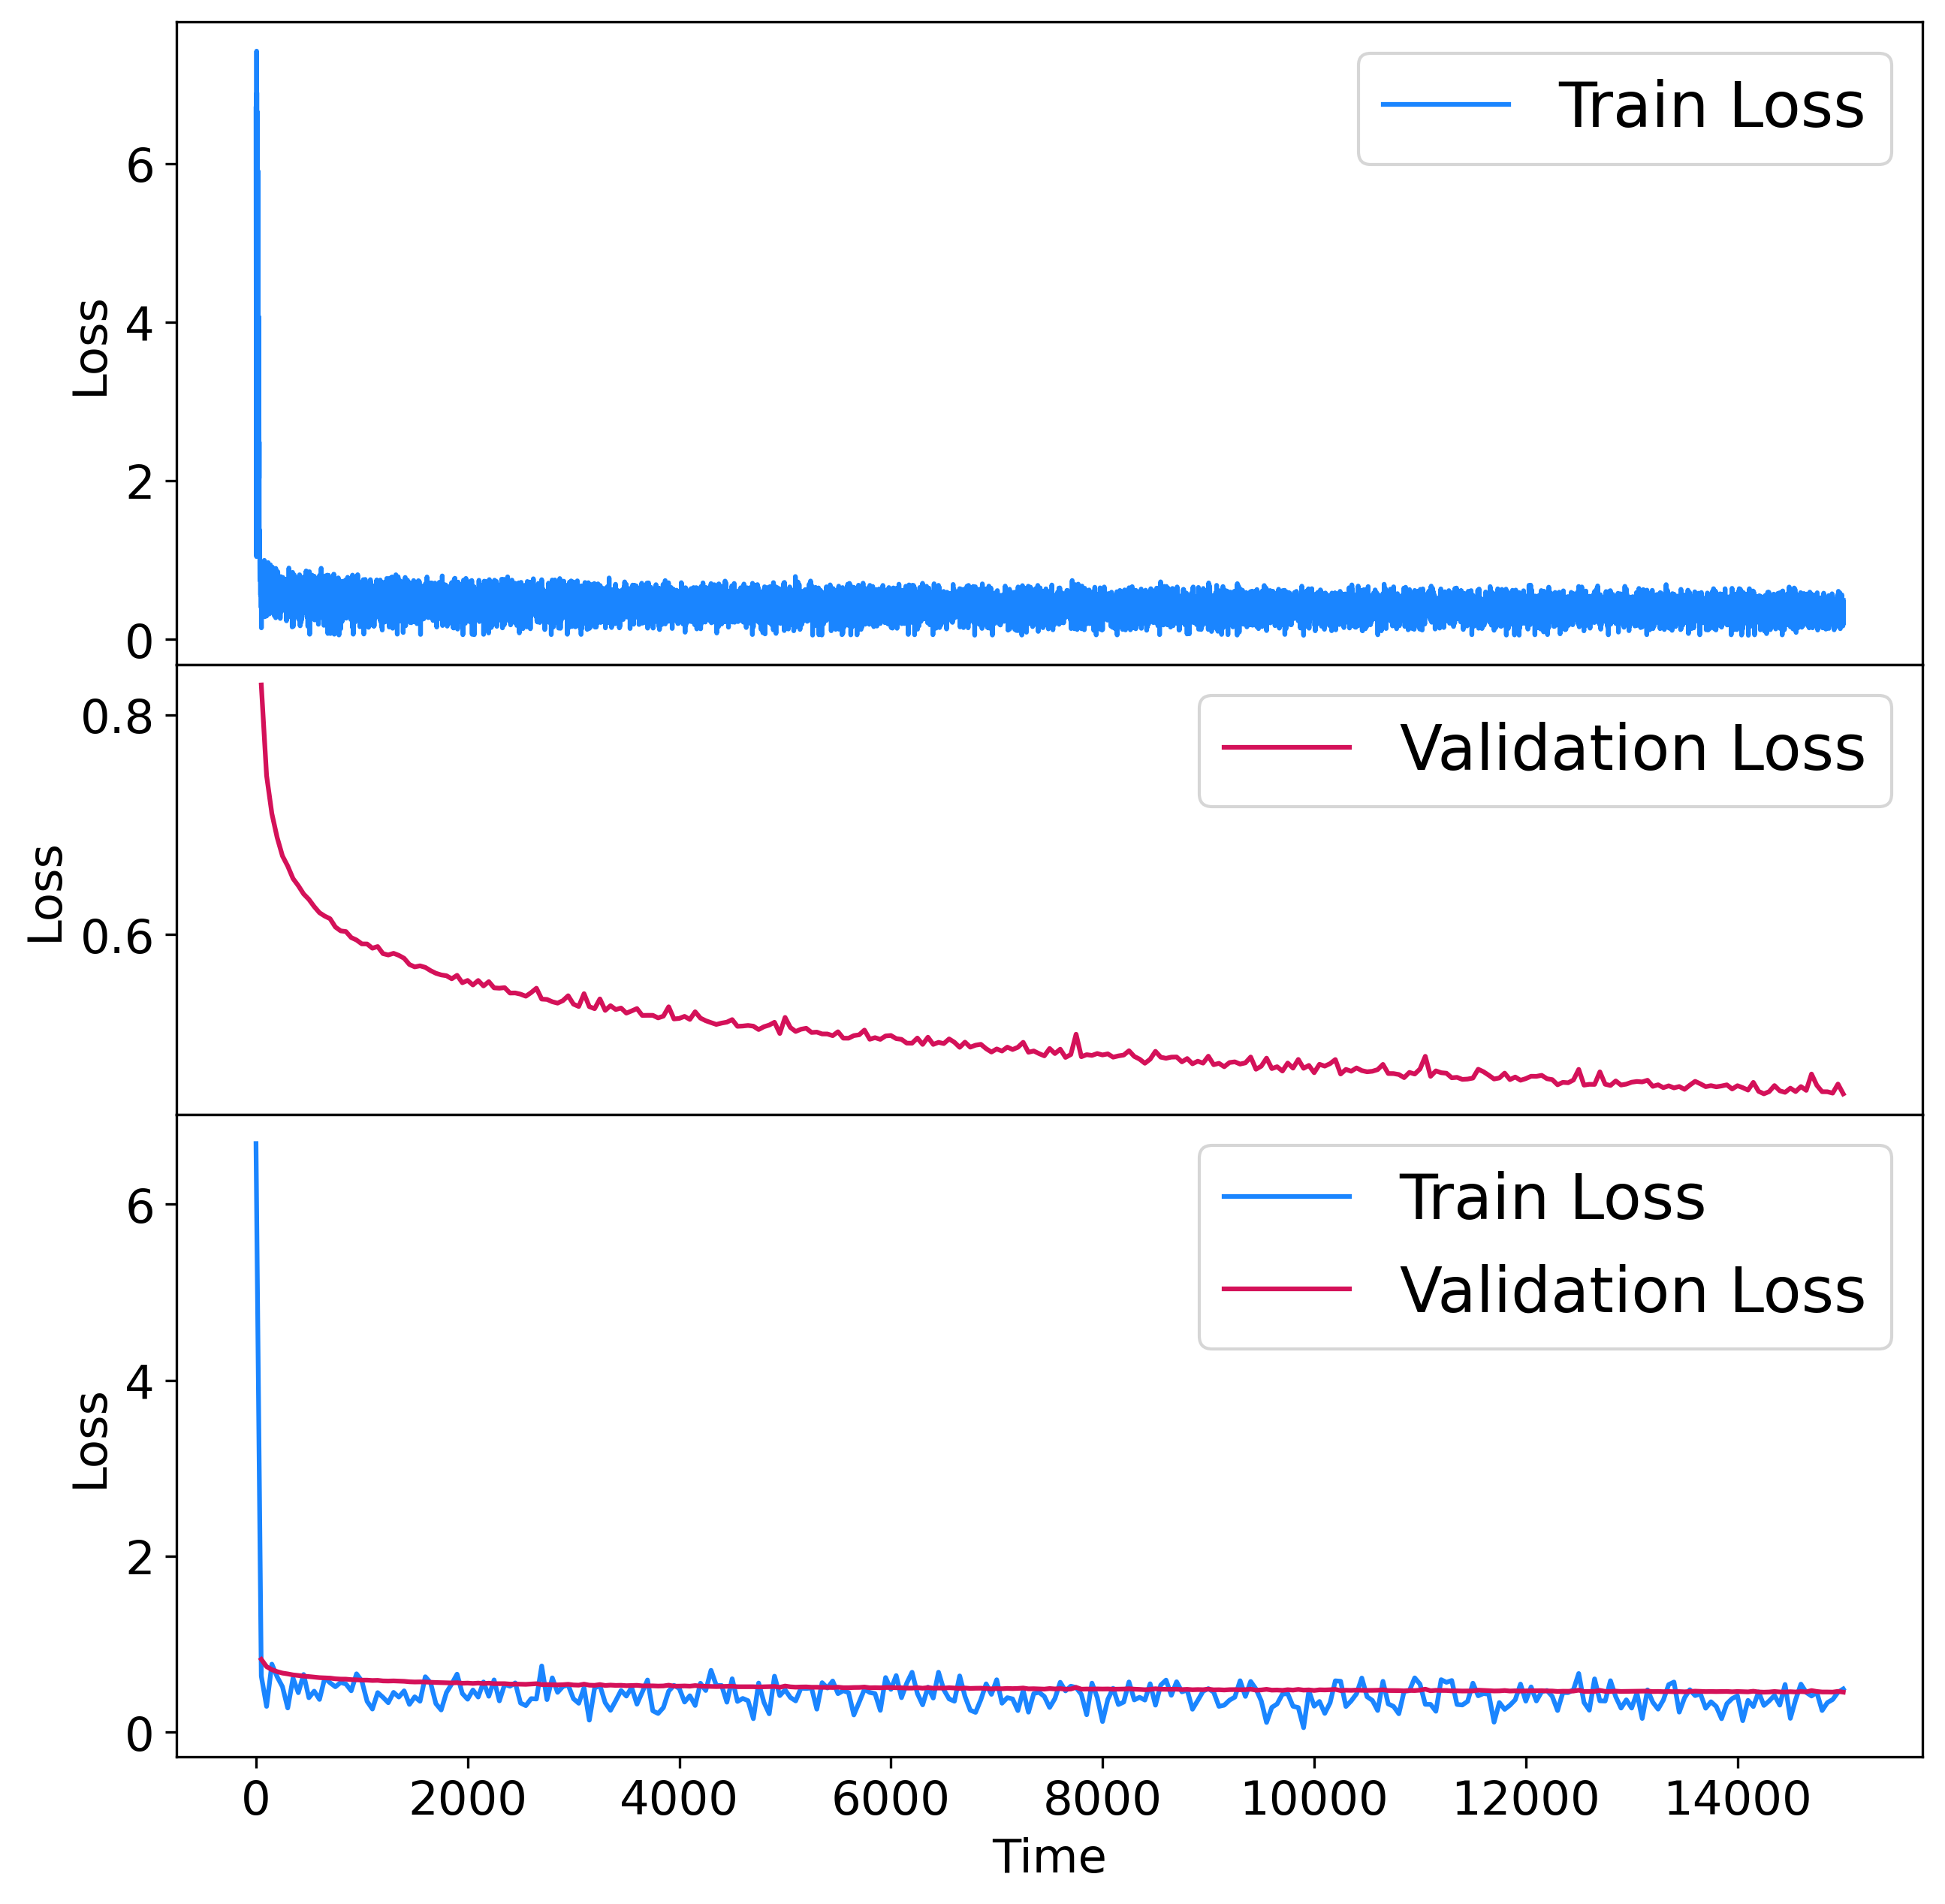
\includegraphics[width=\columnwidth, keepaspectratio]{../plots/lora_final_loss.png}
    \caption{Training (top) and validation (middle) loss for the model fine-tuned with LoRA on the dataset using the final best hyperparameters. The bottom figure directly compares the training (blue) and validation (red) loss using the same resolution of every 50 steps.}
\label{fig:lora_final_loss}
\end{figure}

\begin{figure}
    \centering
    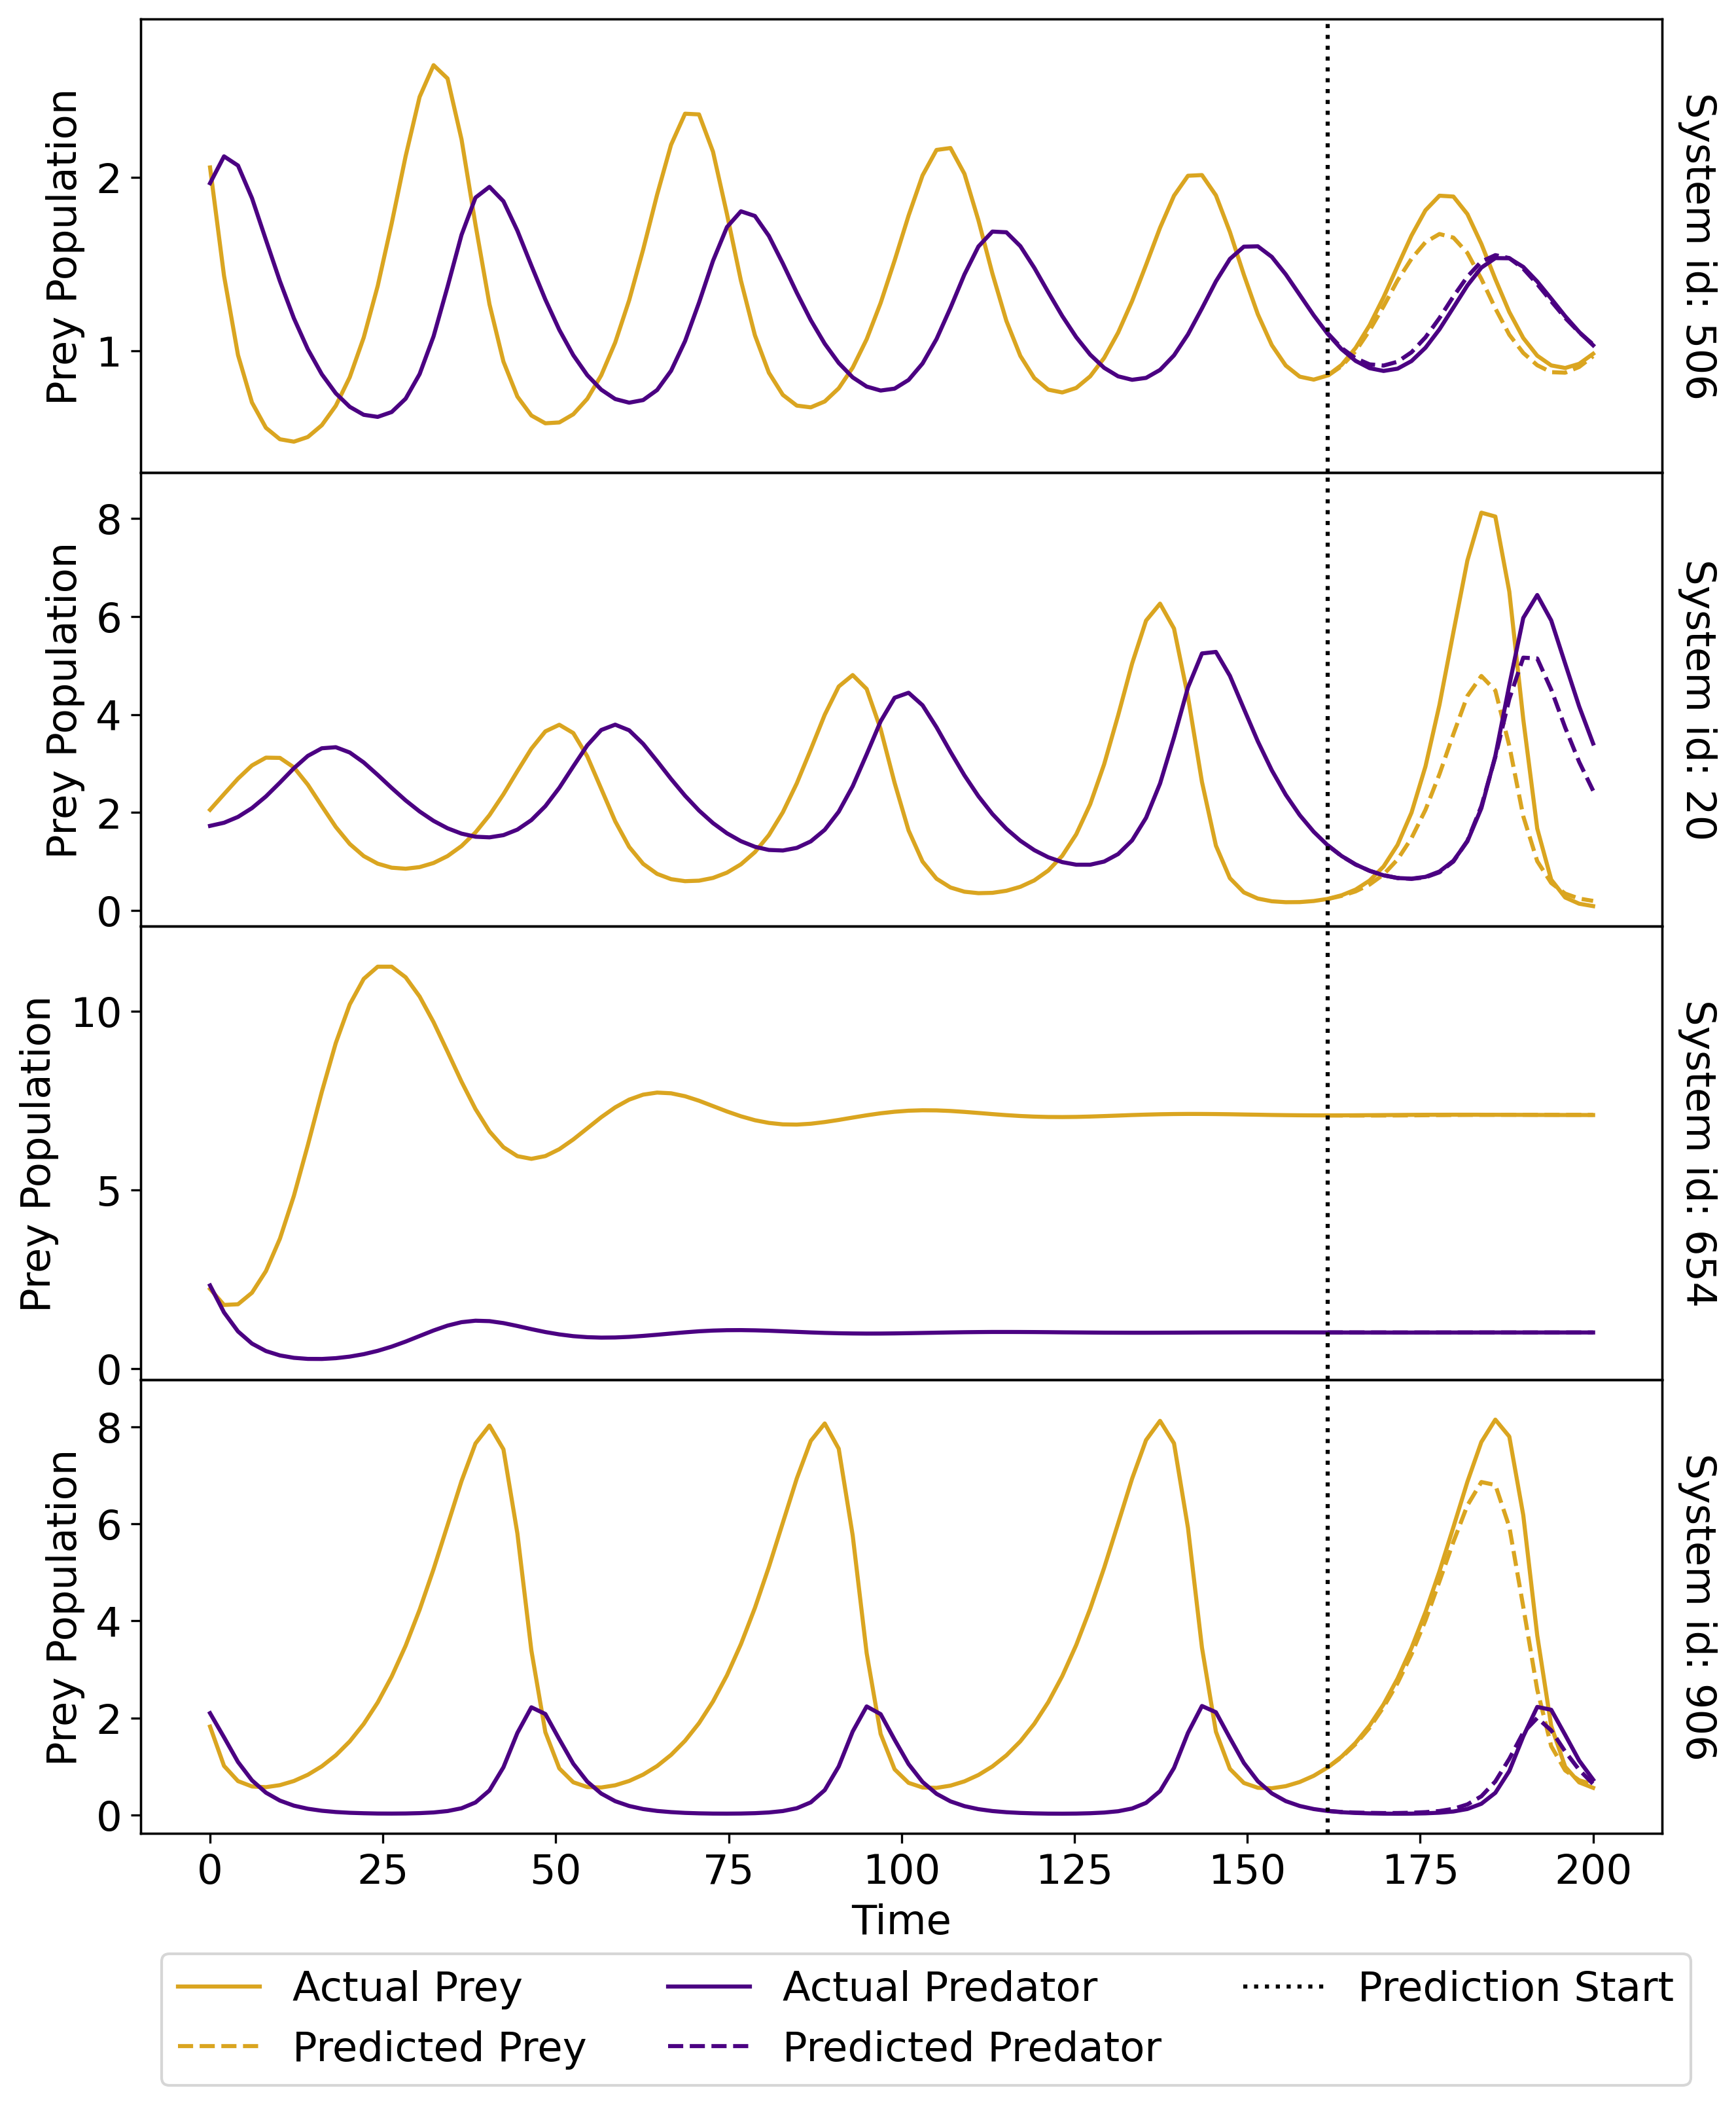
\includegraphics[width=\columnwidth, keepaspectratio]{../plots/predictions_lora_final.png}
    \caption{Predictions (dashed) of the model fine-tuned with LoRA using the final best hyperparameters compared with the true (solid) values on a subset of the test set for both predator (purple) and prey (gold).}\label{fig:lora_final_pred}
\end{figure}

\begin{table}
    \centering
    \begin{tabular}{c|c|c|c|c|c|c|c|c}
        & \multicolumn{2}{c|}{506} & \multicolumn{2}{c|}{20} & \multicolumn{2}{c|}{654} & \multicolumn{2}{|c}{906} \\
        Metric & Prey & Predator & Prey & Predator & Prey & Predator & Prey & Predator \\
        \hline
        MSE & 0.004 & 0.001 & 2.013 & 2.121 & 0.000 & 0.000 & 6.177 & 0.739 \\
        RMSE & 0.064 & 0.024 & 1.419 & 1.456 & 0.012 & 0.001 & 2.485 & 0.859 \\
        MAE & 0.053 & 0.018 & 0.779 & 0.881 & 0.012 & 0.001 & 1.488 & 0.602 \\
        MAPE & 0.041 & 0.015 & 0.232 & 0.231 & 0.002 & 0.001 & 0.325 & 1.887 \\    
    \end{tabular}
    \caption{Metrics for the model fine-tuned with LoRA using the final best hyperparameters on a subset from the test set.}
    \label{tab:lora_final_metrics}
\end{table}

\begin{figure}
    \centering
    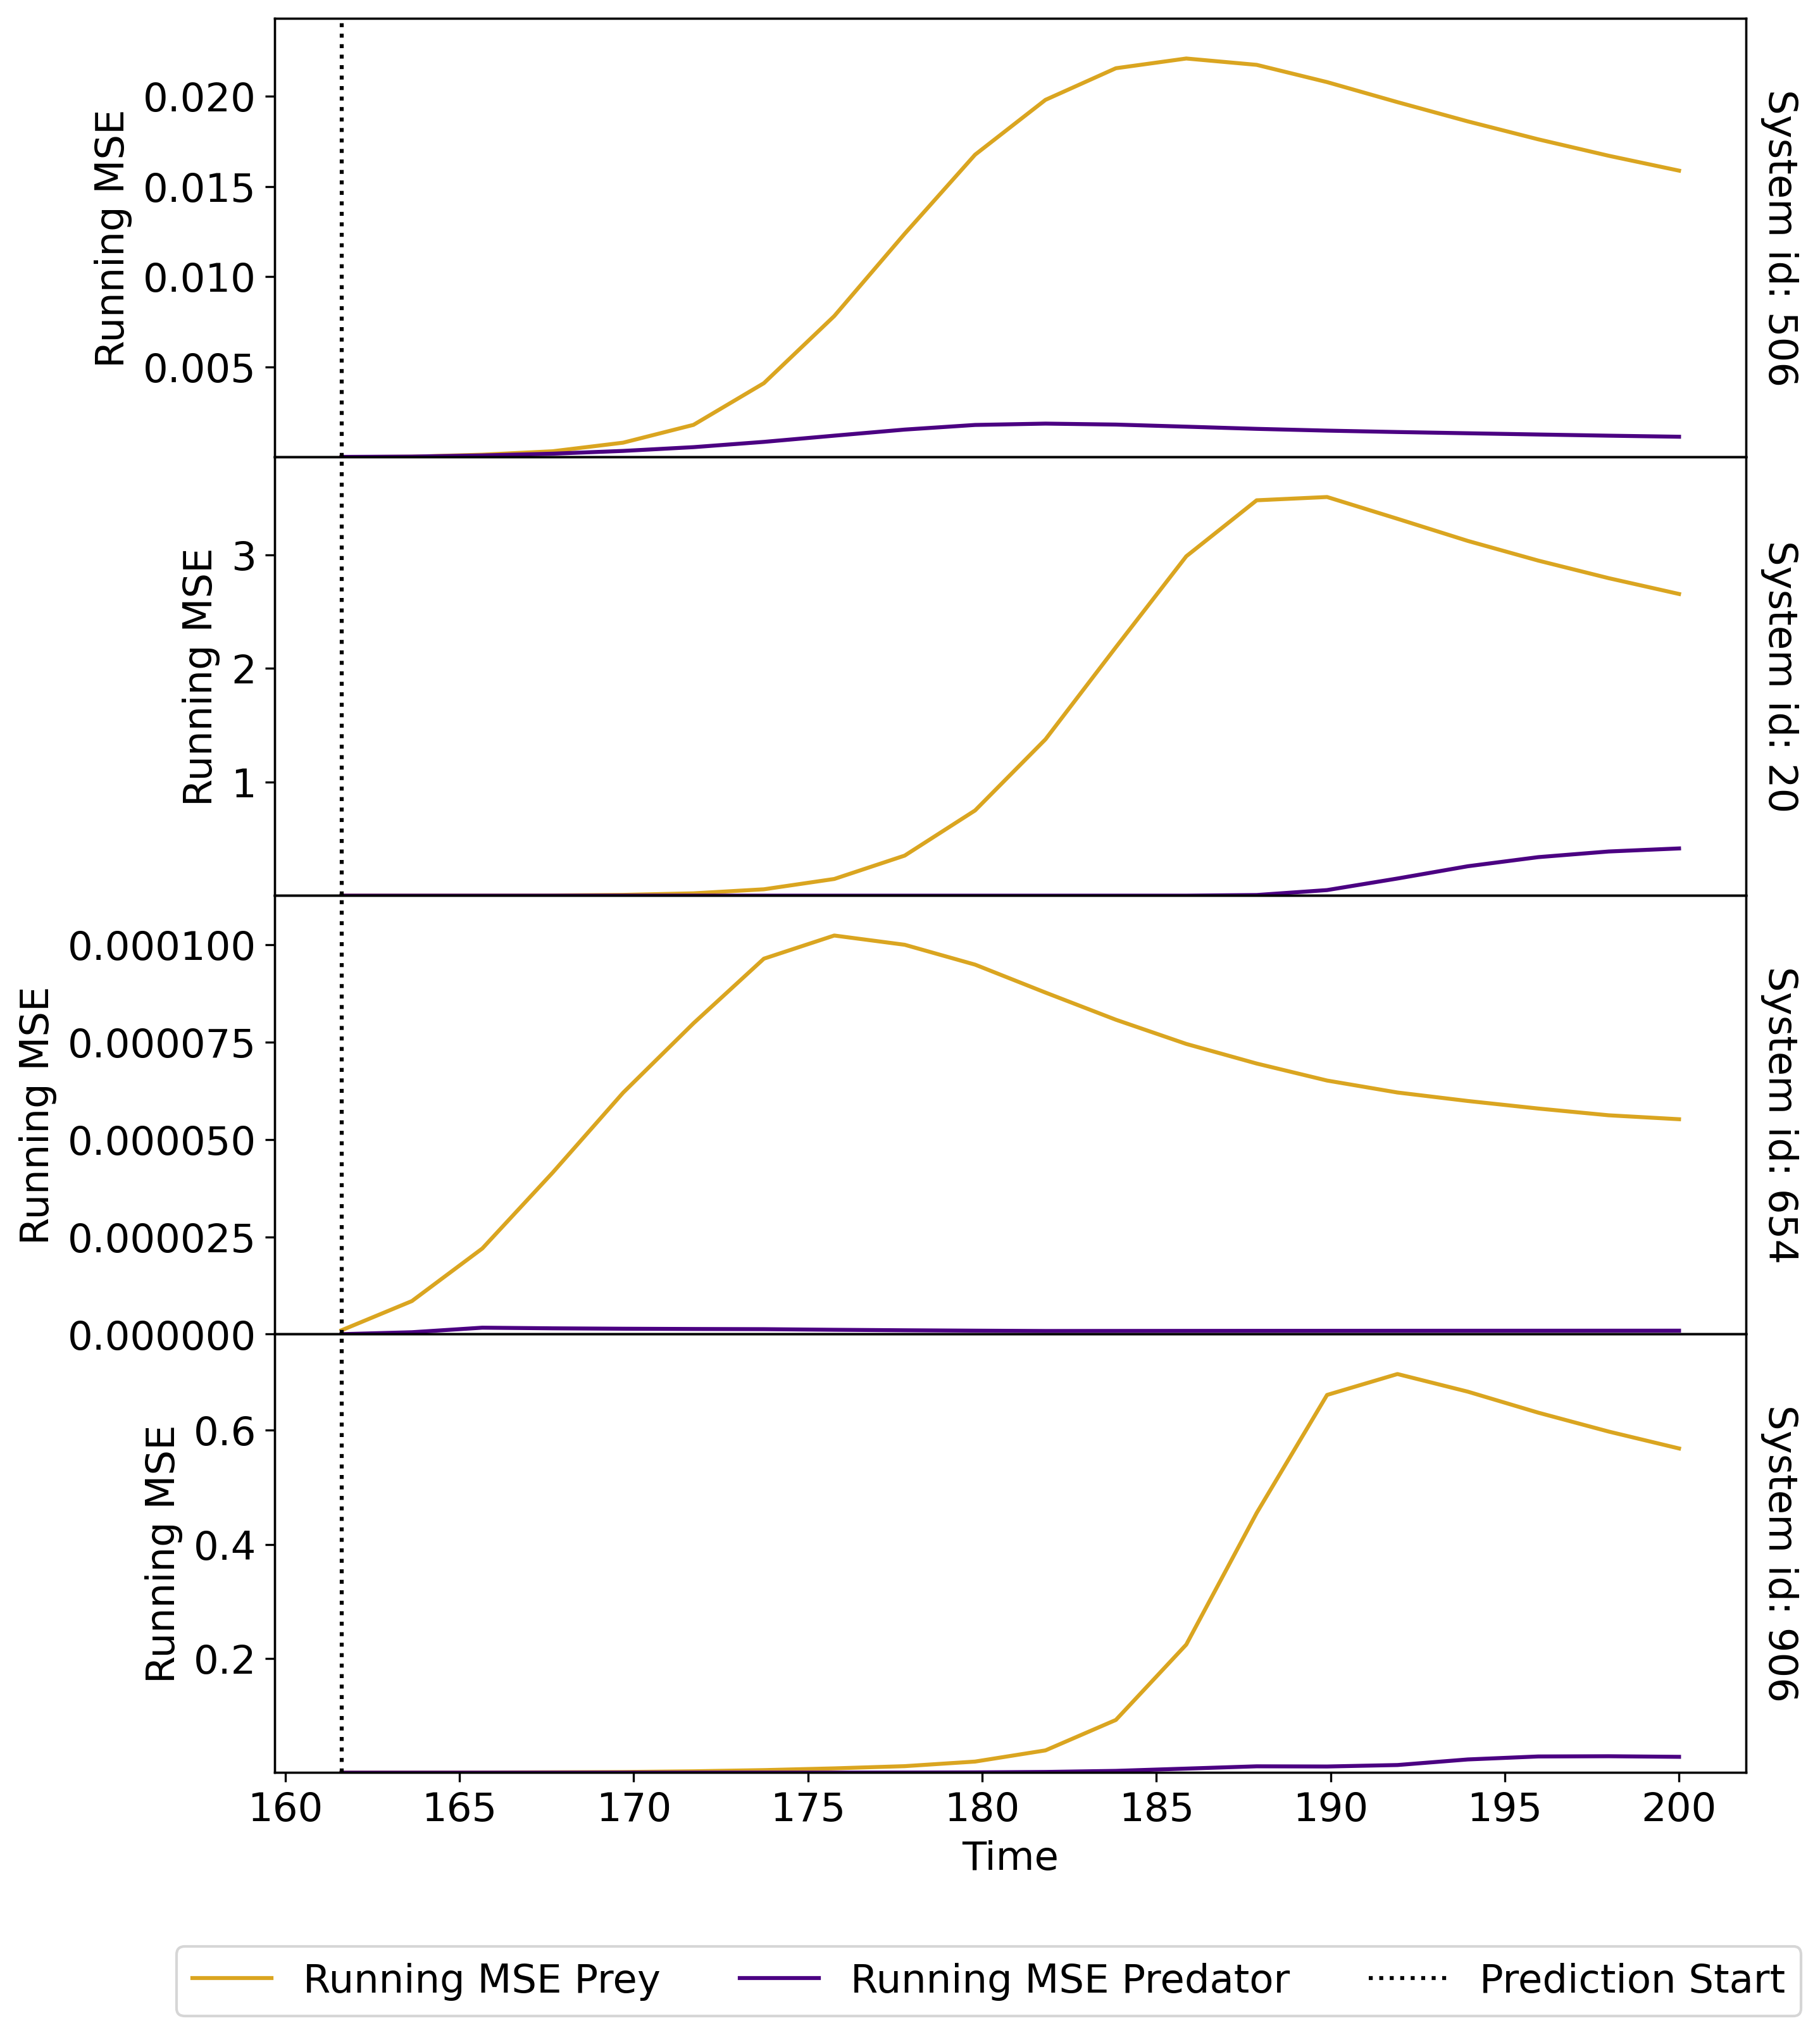
\includegraphics[width=\columnwidth, keepaspectratio]{../plots/running_mse_lora_final.png}
    \caption{Running mean squared error (RMSE) for the model fine-tuned with LoRA using the final best hyperparameters on a subset of the test set over the out-of-distribution data for the predator (purple) and prey (gold) time series.}
    \label{fig:lora_final_rmse}
\end{figure}

As can be seen in Fig.~\ref{fig:lora_final_loss}, the validation loss has not yet plateaued by 15,000 steps, indicating that the model was still learning from the data when training was stopped. However, with deference to the computational constraint of this coursework, the model was not trained for longer.

Comparing Figures \ref{fig:baseline_pred} and \ref{fig:lora_final_pred}, the model's performance on the test set is better than that of the untrained model or the LoRA adapted model trained with the default hyperparameters. This is especially shown by the growing and decaying systems 506 and 20, where the model is now able to predict at least the rough shape of the curve, though not the exact values. The model is also able to predict the overall shape of the oscillatory system 906 fairly well, though not as well as the untrained model. And as the stable system 654 has settled into constant values before the cut-point, the model is able to predict the next 20 points with very small error.

This is also reflected in the metrics shown in Table~\ref{tab:lora_final_metrics}, where the error metrics for all the systems except system 906 have decreased significantly compared to the metrics from Tables~\ref{tab:baseline} and \ref{tab:lora_default_metrics}. In contrast, the errors recorded for system 906 increased significantly once the model was fine-tuned with LoRA, as seen in Table~\ref{tab:lora_default_metrics}. This was improved with hyperparameter tuning and a longer training time, as the model learns to predict Lotka-Volterra time series data. 

\section{FLOPS usage}

The FLOPS used for every experiment are shown in Table~\ref{tab:flops_track}. As can be seen, the coursework is well within the stated budget of $1 \times 10^{17}$ FLOPS.

\begin{table}[h]
    \centering
    \begin{tabular}{c|c|c|c|c}
        & \multicolumn{4}{|c}{FLOPS}\\
        Stage & Training & Validation & Inference & Total \\
        \hline
        Untrained & -- & -- & 5.416e+12 & 5.416e+12 \\
        Default hyperparameters & 9.812e+15 & 1.308e+14 & 5.416e+12 & 9.948e+15 \\
        $\eta$ \& $r$ tuning & 8.831e+15 & 1.177e+14 & -- & 8.948e+15 \\
        Context length tuning & 2.723e+15 & 3.631e+13 & -- & 2.759e+15 \\
        Final run & 9.812e+15 & 1.308e+14 & 5.416e+12 & 9.948e+15 \\
        \hline
        Total & 9.659e+16 & 1.288e+15 & 1.625e+13 & 9.790e+16 \\
    \end{tabular}
    \caption{FLOPS usage for each stage of the coursework including inference by the untrained model; training and inference of the LoRA adapted model with default hyperparameters; grid search of $\eta$, LoRA rank, and context length; and the training and inference of the final model.}
    \label{tab:flops_track}
\end{table}

When fine-tuning models for time-series forecasting under tight budgets, it is recommended to limit the length of training steps. This is because as seen in Sections \ref{sec:lora_lr} and \ref{sec:max_ctx}, it became clear fairly quickly which hyperparameters were best, sometimes being obvious at even just 50 steps. For this coursework, the hyperparameter search runs were done for 300 steps to make sure the inital best hyperparameter stayed as such.

For this coursework, a maximum context length of 512 could have been chosen over that of 768 if the FLOPS budget was becoming a serious concern. This is because as seen in Section \ref{sec:max_ctx}, it performed fairly similarly whilst commanding a lower FLOPS cost.

Another recommendation is to limit the amount of times the validation loss calculation is performed whilst training. It not only takes up more of the FLOPS budget, but also increases the compute time per training run. During this coursework, the validation was computed every 50 steps. This saved FLOPS as well as compute, but also provided enough information to see how the validation loss changed over time.

\section{Further improvements}

As seen in Fig.~\ref{fig:lora_final_pred} in Section \ref{sec:final_model}, the final model still does not predict Lotka-Volterra time series data to a high degree of accuracy for all types of systems. This may be improved by simply increasing the compute by allowing it to train for longer, but there are other optimisations possible.

One way to do this is by considering $\alpha$ as a tunable hyperparameter. According to \citeauthor{hu2021loralowrankadaptationlarge}, it is recommended that $\alpha$ should be around twice the LoRA rank. Throughout this coursework, $\alpha$ was fixed at the LoRA rank, limiting the impact the LoRA weights had on the model's output and how effectively the model learns from the training data, affecting its performance.

Another way to further improve the performance of the model is to include a scheduler. This is because of the problem mentioned in Section \ref{sec:lora_lr}, where a large learning rate showed larger dividends compared to the smaller learning rates. However, with a larger learning rate, it might only show such benefits in only the initial few training steps of the model and in the later stages, a smaller learning rate might prove more beneficial. This is especially obvious in Figures \ref{fig:lora_default_loss} and \ref{fig:lora_final_loss}, where the training and validation loss curves begin to plateau at around 1,000 steps. This is where a scheduler comes in, where $\eta$ of the optimizer is allowed to change over the course of the training run. Some tuning would be required to find the optimal scheduler and parameters for that scheduler, again impacting the FLOPS budget, but that would further improve the performance of the model.

\section{Summary}
The Qwen2.5-0.5B-Instruct LLM was fine-tuned using LoRA matrices and the optimised hyperparameters $\eta$, $r$, and maximum context length. This improved the performance of the model on predicting Lotka-Volterra time series data especially from its default state, but there are several improvements yet to be made.

LLMs may be somewhat competent at time series forecasting, but for more complex systems, it takes a large training dataset and lots of fine-tuning to reach acceptable levels of accuracy.
\clearpage
\bibliographystyle{vancouver-authoryear}
\bibliography{bibliography}
\appendix
\section{Use of auto-generation tools}
Auto-generation tools were used to help parse error messages throughout the project, and to help format this \LaTeX\ report. Auto-generation tools were also used in helping to create a \texttt{move\_to\_cpu} function to move tensors on the GPU to the CPU. Auto-generation tools were also used to help with creating a \texttt{decoding} function that stripped out LLM injected errors in the model's output to transform it into time series arrays.

Auto-generation tools were not used elsewhere, for code generation, writing, or otherwise.
\end{document}
